\documentclass[sigconf,review,anonymous]{acmart}

\usepackage{tablefootnote}
\usepackage{syntax}
\usepackage{multirow}
\usepackage{multicol}
\usepackage{booktabs} % For formal tables
\usepackage{tikz}
\usetikzlibrary{arrows,shadows,positioning,decorations.pathmorphing}
\usepackage{pgf-umlsd}
\usepackage{tikz-uml}
\usepackage{hyperref}
\usepackage{upquote}
\usepackage{listings}
\usepackage{lsthaskell}
\usepackage{xspace}
\usepackage{mdframed}
\usepackage{algorithmic}
\usepackage{longtable}
\usepackage{subcaption}
\usepackage{pgfplots}
\pgfplotsset{compat=newest}
\usepackage[titlenotnumbered, linesnumbered, ruled]{algorithm2e} % language for algorithm description
\hypersetup{
  colorlinks   = true, %Colours links instead of ugly boxes
  urlcolor     = blue, %Colour for external hyperlinks
  linkcolor    = red, %Colour of internal links
  citecolor    = green %Colour of citations
}


%%%%%%%%%%%%%%%%%%%%%%%%%%%%%%%%%%%%%%%%%%%%%%%%%%%%%%%%%%%%%
\definecolor{ltblue}{rgb}{0,0.4,0.4}
\definecolor{dkblue}{rgb}{0,0.1,0.6}
\definecolor{dkgreen}{rgb}{0,0.4,0}
\definecolor{dkviolet}{rgb}{0.3,0,0.5}
\definecolor{dkred}{rgb}{0.5,0,0}

\definecolor{lightgray}{rgb}{0.95, 0.95, 0.95}
\definecolor{darkgray}{rgb}{0.4, 0.4, 0.4}
%\definecolor{purple}{rgb}{0.65, 0.12, 0.82}
\definecolor{editorGray}{rgb}{0.95, 0.95, 0.95}
\definecolor{editorOcher}{rgb}{1, 0.5, 0} % #FF7F00 -> rgb(239, 169, 0)
\definecolor{editorGreen}{rgb}{0, 0.5, 0} % #007C00 -> rgb(0, 124, 0)
\definecolor{orange}{rgb}{1,0.45,0.13}		
\definecolor{olive}{rgb}{0.17,0.59,0.20}
\definecolor{brown}{rgb}{0.69,0.31,0.31}
\definecolor{purple}{rgb}{0.38,0.18,0.81}
\definecolor{lightblue}{rgb}{0.1,0.57,0.7}
\definecolor{lightred}{rgb}{1,0.4,0.5}
% CSS
\lstdefinelanguage{CSS}{
  keywords={color,background-image:,margin,padding,font,weight,display,position,top,left,right,bottom,list,style,border,size,white,space,min,width, transition:, transform:, transition-property, transition-duration, transition-timing-function},	
  sensitive=true,
  morecomment=[l]{//},
  morecomment=[s]{/*}{*/},
  morestring=[b]',
  morestring=[b]",
  alsoletter={:},
  alsodigit={-}
}

% JavaScript
\lstdefinelanguage{JavaScript}{
  morekeywords={typeof, new, true, false, catch, function, return, null, catch, switch, var, if, in, while, do, else, case, break, for},
  morecomment=[s]{/*}{*/},
  morecomment=[l]//,
  morestring=[b]",
  morestring=[b]'
}

\lstdefinelanguage{HTML5}{
  language=html,
  sensitive=true,	
  alsoletter={<>=-},	
  morecomment=[s]{<!-}{-->},
  morestring=[b]'
  tag=[s],
  otherkeywords={
  % General
  >,
  % Standard tags
	<!DOCTYPE,
  </html, <html, <head, <title, </title, <style, </style, <link, </head, <meta, />,
	% body
	</body, <body,
	% Divs
	</div, <div, </div>, 
	% Paragraphs
	</p, <p, </p>,
	% scripts
	</script, <script,
  % More tags...
  <canvas, /canvas>, <svg, <rect, <animateTransform, </rect>, </svg>, <video, <source, <iframe, </iframe>, </video>, <image, </image>, <header, </header, <article, </article
  },
  ndkeywords={
  % General
  =,
  % HTML attributes
  charset=, src=, id=, width=, height=, style=, type=, rel=, href=,
  % SVG attributes
  fill=, attributeName=, begin=, dur=, from=, to=, poster=, controls=, x=, y=, repeatCount=, xlink:href=,
  % properties
  margin:, padding:, background-image:, border:, top:, left:, position:, width:, height:, margin-top:, margin-bottom:, font-size:, line-height:,
	% CSS3 properties
  transform:, -moz-transform:, -webkit-transform:,
  animation:, -webkit-animation:,
  transition:,  transition-duration:, transition-property:, transition-timing-function:,
  }
}

\lstdefinelanguage{HTML5}{
  language=html,
  tagstyle=\color{blue},
  markfirstintag=true,
  sensitive=true,
  alsoletter={<>=-},	
  morecomment=[s]{<!--}{-->},
  % tag=[s],
  %% morestring=[b]'',
  morestring=[b]',
  ndkeywords={
    % General
    =,
    % HTML attributes
    id=, class= 
  }
}


\lstdefinestyle{htmlcssjs} {%
  % General design
  backgroundcolor=\color{editorGray},
  basicstyle={\scriptsize\ttfamily},   
  frame=tb,
  % line-numbers
  xleftmargin={0.75cm},
  numbers=left,
  stepnumber=1,
  firstnumber=1,
  numberfirstline=true,	
  % Code design
  identifierstyle=\color{black},
  keywordstyle=\color{blue}\bfseries,
  ndkeywordstyle=\color{editorGreen}\bfseries,
  stringstyle=\color{editorOcher}\ttfamily,
  commentstyle=\color{brown}\ttfamily,
  % Code
  language=JavaScript,
  alsolanguage=HTML5,
  alsodigit={.:;},	
  tabsize=2,
  showtabs=false,
  showspaces=false,
  showstringspaces=false,
  extendedchars=true,
  breaklines=true,
  escapechar=|c
}
%%%%%%%%%%%%%%%%%%%%%%%%%%%%%%%%%%%%%%%%%%%%%%%%%%%%%%%%%%%%%

\listfiles % used to output the versions of all files being used by the latex

\newcommand{\Server}{\emph{Server}\xspace}
\newcommand{\Client}{\emph{Client}\xspace}
\newcommand{\User}{\emph{User}\xspace}
\newcommand{\Validator}{\emph{Validator}\xspace}
\newcommand{\thenBr}{\text{then}}
\newcommand{\elseBr}{\text{else}}
\newcommand{\inFor}{\text{inFor}}
\newcommand{\inWhile}{\text{while}}
\newcommand{\un}[1]{\underline{#1}}
\newcommand{\Random}{\mathbb{R}}
\newcommand{\Genetic}{\mathbb{G}}
\newcommand{\RGenetic}{\mathbb{G}_{10}}

% Copyright
\setcopyright{none}
%\setcopyright{acmcopyright}
%\setcopyright{acmlicensed}
%\setcopyright{rightsretained}
%\setcopyright{usgov}
%\setcopyright{usgovmixed}
%\setcopyright{cagov}
%\setcopyright{cagovmixed}


% DOI
%\acmDOI{10.475/123_4}

% ISBN
%\acmISBN{123-4567-24-567/08/06}

%Conference
\acmConference[ISSTA 2018]{ACM SIGSOFT International Symposium on Software Testing and Analysis}{16-22 July, 2018}{Amsterdam, The Netherlands}
%% \acmYear{1997}                  
%% \copyrightyear{2016}

%% \acmPrice{15.00}

\begin{document}
\title{Search-Based Test Data Generation for JavaScript Functions with DOM}


\author{Alexander Elyasov}
\affiliation{%
  \institution{Utrecht University, The Netherlands} 
}
\email{a.elyasov@uu.nl}

\author{Wishnu Prasetya}
\affiliation{%
  \institution{Utrecht University, The Netherlands}
}
\email{s.w.b.prasetya@uu.nl}

\author{Jurriaan Hage}
\affiliation{%
  \institution{Utrecht University, The Netherlands}
  \country{The Netherlands} 
}
\email{j.hage@uu.nl}


\begin{abstract}
As of 2017 JavaScript and Node.js continue to stay the most prevalent technologies according to the Stack Overflow developers survey. Nevertheless, existing JS testing frameworks are still lacking any support for such a vital step in test automation as the generation of input data. To address this problem, we present a novel \textbf{J}avascript \textbf{E}volutionary-based testing framework with \textbf{D}OM as an \textbf{I}input, called \textbf{JEDI}. In order to reach a target branch, it applies genetic search for relevant input parameters of the JS function including global DOM state. The \emph{genetic with restart} algorithm, proposed in this paper, was able to achieve complete branch coverage in our empirical evaluation with the average execution time 7.7 sec. per branch 
\end{abstract}

%
% The code below should be generated by the tool at
% http://dl.acm.org/ccs.cfm
% Please copy and paste the code instead of the example below. 
%
\begin{CCSXML}
<ccs2012>
<concept>
<concept_id>10011007.10011074.10011099.10011102.10011103</concept_id>
<concept_desc>Software and its engineering~Software testing and debugging</concept_desc>
<concept_significance>300</concept_significance>
</concept>
<concept>
<concept_id>10011007.10011074.10011784</concept_id>
<concept_desc>Software and its engineering~Search-based software engineering</concept_desc>
<concept_significance>300</concept_significance>
</concept>
</ccs2012>
\end{CCSXML}

\ccsdesc[300]{Software and its engineering~Software testing and debugging}
\ccsdesc[300]{Software and its engineering~Search-based software engineering}

\keywords{JavaScript, search-based testing, branch coverage}


\maketitle


\section{Introduction}
\label{sec.intro}

According to a Stack Overflow survey\footnote{\url{https://insights.stackoverflow.com/survey/2017}} run in 2017 across developers, JavaScript has been recognized for the fifth time in row as the most commonly used programming language with Node.js as the most commonly used technology. It is used through all technology stack web, back-ends and mobile. Such a tremendous ever increasing JS success is happening thanks to the extensive dynamic features of the language, JS permissiveness and native browser support. On the other hand, JS applications are error-prone~\cite{why}, hard to analyze~\cite{why} and test~\cite{why}. Therefore, it is not surprising that year after year we hear new stories\footnote{\url{https://www.fastcompany.com/40505226/the-year-that-software-bugs-ate-the-world}} about another critical bug being found in a web application by Facebook, Twitter etc. 

%% Common mistakes JS developers do\footnote{\url{https://www.toptal.com/javascript/10-most-common-javascript-mistakes}}.

%% Notable errors in 2017\footnote{\url{https://www.fastcompany.com/40505226/the-year-that-software-bugs-ate-the-world}}. 

The state of JS 2017 survey~\footnote{\url{https://stateofjs.com/}} contains an extensive list of testing frameworks including Mocha, Jasmine, Jest, Enzyme, Tape, Ava, Karma and QUnit. These frameworks support testing at various levels: unit, integration and functional. The survey also indicated relatively low satisfaction rate of the current state of JS testing tools, scoring only 3.2 out of 5. As result, new testing frameworks such as Cypress and Storybook are constantly appearing to improve the situation. But despite of this effort, test data generation continues to be not properly addressed by any of the widely used testing frameworks. The research community has actively been working towards making progress in this direction introducing such tools as Artemis~\cite{artemis2011}, JSConTest~\cite{heidegger2010contract}, Crawljax~\cite{mesbah2012crawling}, JSeft~\cite{mirshokraie2015jseft} and Jalangi~\cite{sen2013jalangi}. A recent study of client-side JS bugs~\cite{ocariza2017study} has shown that the majority (68\%) of JS faults are DOM-related and occur in JS code, and not in HTML or CSS. This fact indicates that yet a better testing approach is needed when it comes to unit testing of JS.

Over the past two decades search-based test data generation has proven to be one of the most effective solutions for a wide range of technologies including object-oriented~\cite{paper}, web~\cite{paper} and mobile~\cite{paper}. In recent years, some effort was made to apply search-based testing to dynamic languages such as Python~\cite{paper}, Ruby~\cite{paper} (maybe mention Go and Lua), but to the best of our knowledge search-based testing approach has never been applied to JavaScript. Our work makes the following contributions:
\begin{enumerate}
\item The \emph{JEDI} framework is a novel JS unit testing tool using search-based techniques for generating test data. Notably, our testing framework is able to generate an arbitrary DOM input, which is syntactically valid and compliant with the recent HTML5 specification.   
\item We propose a novel test generation algorithm, called ``genetic with restart'', combining the benefits of systematic fitness improvement with the genetic search and the ability of escaping plateau by restarting search with a new target.
\item Based on the case studies found in two related works~\emph{Confix}~\cite{amin:ase15} and \emph{TAJS}~\cite{dom2011}, we conduced an empirical validation of our framework and performed a significance study of the results. The validation has shown the effectiveness of the framework in covering target branches with a reasonable efficiency...  
\end{enumerate} 

The paper is structured as follows: In Section~\ref{sec.example}, we present a motivating example illustrating the challenges of generating test data for JS. The architecture of the \emph{JEDI} testing framework is explained in Section~\ref{sec.framework}. Section~\ref{sec.evaluation} present empirical validation, whereas Section~\ref{sec.disc} discusses future work and validity threats. We discuss related work in Section~\ref{sec:related.work} and conclude the paper in Section~\ref{sec:concl}.  

Another empirical work~\cite{richards2010analysis}.

%% --------------------------------------------------------------------
\section{Motivating Example}
\label{sec.example}
%% --------------------------------------------------------------------

\begin{figure}[t]
  \begin{lstlisting}[style=htmlcssjs,language=JavaScript]
/*t dom */
function isGameFinished() {
  var obj = document.getElementById('sudoku'); |c \label{isGameFinished.getSudoku} |c
  var subDivs = obj.getElementsByTagName('DIV'); |c \label{isGameFinished.getDivs} |c
  var allOk = true;
  for (var no = 0; no < subDivs.length; no++) { |c \label{isGameFinished.inFor.begin} |c
    if (subDivs[no].className.indexOf('sudokuSquare') >= 0 |c \label{isGameFinished.if1.begin} |c 
        && !subDivs[no].style.backgroundColor) { 
      var spans = subDivs[no].getElementsByTagName('SPAN');
      if (spans[0].innerHTML != spans[1].innerHTML) { |c \label{isGameFinished.if2.begin} |c
        allOk = false; |c \label{isGameFinished.unfinished} |c
        break; 
      }
    }
  } |c \label{isGameFinished.outFor} |c
}
\end{lstlisting}
  \caption{JS function \texttt{isGameFinished.js} from sudoku}
  \label{code.isGameFinished}
\end{figure}

\begin{figure}[t]
  \begin{lstlisting}[style=htmlcssjs, language=HTML5]
<!-- T1: (5,5) -->            <!-- T2: (5,6), (7,15) -->
<html>                        <html>
 <body>                        <body>
  <div id='sudoku'>             <div id='sudoku'>
                                 <div></div>                           
  </div>                        </div> 
 </body>                       </body>    
</html>                       </html>  

<!-- T3: (7,8), (10,14) -->   <!-- T4: (7,8), (10,11) -->
<html>                        <html>
 <body>                        <body>
  <div id='sudoku'>             <div id='sudoku'>
   <div class='sudokuSquare'>    <div class='sudokuSquare'>
    <span></span>                 <span></span> 
    <span></span>                 <span>TEST</span>
   </div>                        </div> 
  </div>                        </div>
 </body>                       </body>
</html>                       </html>
  \end{lstlisting}
  \caption{Input DOM arguments for \texttt{isGameFinished.js}}
  \label{fig.isGameFinished.tests}
\end{figure}

Let us consider the JS function \texttt{isGameFinished} in Figure~\ref{code.isGameFinished} taken from a web game \emph{sudoku}\footnote{\url{http://www.dhtmlgoodies.com/scripts/game_sudoku/game_sudoku.html}}. This function checks the validity of a sudoku solution given by a user. First, we find a DOM element representing the game field (line~\ref{isGameFinished.getSudoku}). Then, we collect all its child DIVs (line~\ref{isGameFinished.getDivs}). Each DIV element corresponds to a sudoku input square (line~\ref{isGameFinished.if1.begin}) and consists of two SPANs. First span contains a user input, whereas the second one, which is hidden by default, stores the expected value for that sudoku square. Inside of a for-loop in lines~\ref{isGameFinished.inFor.begin}-\ref{isGameFinished.outFor}, we iterate over the whole collection of input squares. Once, we find a square with two unequal SPAN values (line~\ref{isGameFinished.if2.begin}), the loop is terminated and the game is considered unfinished (line~\ref{isGameFinished.unfinished}) and finished otherwise.

Suppose now that we would like to unit test this function in isolation to the rest of the application. We aim to maximize the branch coverage as a common testing criteria~\cite{why.this.common}. That is, for each individual branch of the function under test (FUT) \texttt{isGameFinished}, we need to construct a test input that covers the branch and leads to the normal termination of the FUT. JS function takes \emph{explicit} input arguments (in our case none), but it can also accept \emph{implicit} arguments such as the DOM state. We assume that DOM is the only global variable that can be referenced in the body of the FUT. So in order to produce a complete test for our function we have to construct both an appropriate DOM and input arguments.   

%Our program has the following branches: $(6,15)$, $(6,7)$, $(7,9)$, $(7,14)$, $(10,11)$, $(10,13)$, $(16,17)$, $(16,18)$. Four tests in 

Figure~\ref{fig.isGameFinished.tests} presents four tests that together deliver the full coverage of the FUT. Let us look now at how following the structure of the FUT in Figure~\ref{code.isGameFinished}, we can construct the $T4$ test covering the $(10,11)$ branch. Line~\ref{isGameFinished.getSudoku} expects the input DOM to have an element with the id \textquotesingle\texttt{sudoku}\textquotesingle. In order to enter the for-loop in line~\ref{isGameFinished.inFor.begin}, that element should have at least one child \emph{DIV} tag. The first if-condition in line~\ref{isGameFinished.if1.begin} requires this $div$ to be of the class \textquotesingle\texttt{sudokuSquare}\textquotesingle\ and also have no background color. The second if-condition (line~\ref{isGameFinished.if2.begin}) expects that the $div$ consists of two \emph{SPAN} elements whose \emph{innerHtml} values are not equal. The resulted test $T4$ is shown in Figure~\ref{fig.isGameFinished.tests} and meets all the above conditions. 

As we have just seen, even for such a relatively simple example, the construction procedure of a test input is far from trivial because it requires the deep understanding of the program semantics. In practice, web developers often have to deal with the gazillion of the JS frameworks and libraries freely available on the GitHub whose code is commonly untested and poorly documented. At the same time, unit testing is the most fundamental level of testing and, at the same time, it is easiest to implement. It greatly saves the developers from unexpected regression and puts a safety belt around the application.

%% --------------------------------------------------------------------
\section{Test Generation Framework}
\label{sec.framework}
%% --------------------------------------------------------------------

\begin{figure}[t!]
  \centering 
  \begin{sequencediagram}[font=\scriptsize]

    \renewcommand\unitfactor{0.35}
    \newinst{user}{\textbf{User}}
    \newinst{server}{\textbf{Server}}
    \newinst[1]{validator}{\textbf{Validator}}
    \newinst{client}{\textbf{Client}}
    
    \begin{call}{user}{fun.js + config}{server}{\textbf{end}}
      \begin{call}{server}{Initialize(fun.js)}{server}{(cfg, branches, cinfo, ifun, sig)}
      \end{call}
      
      \begin{call}{server}{POST /init \{ifun, sig\}}{client}{status}
      \end{call}
      
      \begin{call}{server}{Select(branches)}{user}{$\text{branches}'$}       
      \end{call}
      
      \begin{sdblock}{\textbf{Genetic Loop}}{\scriptsize \hspace{8mm}$\text{branch} \in \text{branches}'$}
        \begin{sdblock}{\textbf{Random Loop}}{\scriptsize errors > 0}
          \begin{call}{server}{pop = Random(cinfo, config)}{validator}{errors}
          \end{call}
          \prelevel
        \end{sdblock}
        
        \begin{sdblock}{\textbf{Fitness Loop}}{\scriptsize (fitness $\neq$ 0) $\vee$ gen.limit}

          \begin{sdblock}{\textbf{Evaluation Loop}}{\scriptsize p $\in$ pop}
            \begin{call}{server}{POST /genetic \{p\}}{client}{response = ifun(p: sig)}
            \end{call}
            
            \begin{callself}{server}{Evaluate(branch, cfg, response)}{fitness}
            \end{callself}
            \prelevel
          \end{sdblock}
          
          \begin{sdblock}{\textbf{Crossover Loop}}{\scriptsize errors > 0}
            \begin{call}{server}{cross = Crossover(cinfo, pop)}{validator}{errors}
            \end{call}
            \prelevel
          \end{sdblock}

          \begin{sdblock}{\textbf{Mutation Loop}}{\scriptsize errors > 0}
            \begin{call}{server}{mut = Mutation(cinfo, pop)}{validator}{errors}
            \end{call}
            \prelevel
          \end{sdblock}
         
          \begin{callself}{server}{pop = cross $\cup$ mut}{pop}
          \end{callself}
          \prelevel
        \end{sdblock}
        \mess{server}{best fitness}{user}
        
      \end{sdblock}
    \end{call}
  \end{sequencediagram}
  \caption{The architecture of the test framework}
  \label{fig.framework.architect} 
\end{figure}

Given a JS function $f$ and a set of branches $\mathbb{B}_f$, the ultimate goal of the testing framework is to find input arguments for $f$ that cover all branches from $B_f$. Our JS testing framework, called \emph{JEDI}, is a client-server application which under the hood uses the genetic engine for test generation. The general workflow of the framework is depicted as a sequence diagram in Figure~\ref{fig.framework.architect}. The diagram consists of the four interacting components \User, \Server, \Validator, and \Client. \Server is the key component of the whole framework. It is responsible for the \emph{Initialization Phase} and the \emph{Genetic Phase}. Both phases will be covered in details in Section~\ref{sub.sec.init.phase} and \ref{sub.sec.genetic.phase} respectively.

Each newly constructed HTML document has to be processed by the \Validator\footnote{\url{https://validator.w3.org/nu/}} which checks its syntactic correctness and reports back the set of identified errors. \Server rejects the document if any errors were revealed and generates a new one until the generated document has no errors anymore. \Client is a \emph{Node.js}\footnote{\url{https://nodejs.org/en/}} application that is mainly responsible for the execution of the JS code. We use the \emph{jsdom}\footnote{\url{https://github.com/tmpvar/jsdom}} library to model the virtual DOM and simulate the native browser API calls.   

Let us give a closer look at the sequence of interactions in Figure~\ref{fig.framework.architect}. As an input for our testing framework, \User has to provide the JS file \emph{fun.js} that contains the function under test (FUT) \emph{fun} annotated with the type signature. Additionally, \User specifies a configuration file \emph{config} that defines various parameters for random data generation, genetic phase, logging etc. Experimentally, we have found an optimal set of input configurations that was used across all experimental objects in Section~\ref{sec.evaluation}. This data is processed by the \Server during the \emph{Initialization Phase}. As an output, we get back the following information about \emph{fun}: the control flow graph (\emph{cfg}), the complete list of its branches (\emph{branches}), the constant info (\emph{cinfo}), the instrumented version \emph{ifun}, and the signature (\emph{sig}). \Server sends a \texttt{POST} request with \emph{ifun} and \emph{sig} to the \Client. Depends on the configured execution mode, the \Server either asks the \User to select a \emph{target} branch or covers all branches one by one in a fixed order. For each branch, our framework enters the \emph{Genetic Loop (Phase)}. Inside of this phase, the framework starts with a randomly generated population (\emph{Random Loop}), and continues to evolve that population (\emph{Fitness Loop}) until either a perfect entity is found or a certain termination criteria is achieved, e.g. the limit on the number of generation attempts. Each candidate in the population has to be evaluated in \emph{Evaluation Loop} by \Client. It matches the candidate $p$ according to the type signature \emph{sig} and invokes the instrumented JS function on it: \emph{ifun(p)}. The execution trace along with some supplementary information about the execution are sent back to the \Server, where the final \emph{fitness value} is computed. The new population is constructed by combining the results of the \emph{Crossover} and \emph{Mutation Loops}. If a new HTML document is produced somewhere in the genetic phase, it has to be first approved by the \Validator. At the end of the \emph{Fitness Loop}, the candidate with the ``best'' fitness value is reported back to the \User. Once all the branches are exercised, the algorithm reaches the end. In the follow up two sections, we elaborate on the details of each individual phase of our test generation framework.

\subsection{Initialization Phase}
\label{sub.sec.init.phase}

\begin{algorithm}[t!]
  \caption{Initialization Phase}
  \label{alg.init}
  \algsetup{linenosize=\tiny}
  \scriptsize
  \DontPrintSemicolon
  \SetAlgoVlined
  \SetKwInOut{Input}{Input}
  \SetKwInOut{Output}{Output}
  \SetKwInOut{Require}{Require}
  \SetKwProg{Fn}{Function}{}{}
  \Input{JS file $fun.js$ with FUT and type annotation }
  \Output{Tuple $(cfg, branches, cinfo, ifun, sig)$}
  \Fn{$Initialize(fun.js)$}{
 
    $(ast, sig) \longleftarrow ParseFuncAndSig(fun.js)$\label{alg.init.parse.fun.sig}\;
    $cinfo \longleftarrow GetConstantInfo(ast)$\label{alg.init.collect.info}\;
    $nast \longleftarrow NormalizeAST(ast)$\label{alg.init.transform.ast}\;
    $ifun \longleftarrow Instrument(nast)$\label{alg.init.instr}\;
    $cfg \longleftarrow BuildCFG(nast)$\label{alg.init.build.cfg}\;
    $branches \longleftarrow GetBranches(cfg)$\label{alg.init.get.branches}\;
    \Return{$(cfg, branches, cinfo, ifun, sig)$}
    }
\end{algorithm}

During the \emph{Initialization Phase} we analyze the FUN in order to retrieve the data required for the consecutive genetic testing. The main steps of this phase are illustrated by Algorithm~\ref{alg.init}. Given a FUT \emph{fun.js} as an input, we parse the function and its type signature in line~\ref{alg.init.parse.fun.sig}. In order to maximize the chances of generating the fittest candidate in the genetic phase, in line~\ref{alg.init.collect.info} we perform static analysis of the FUT with the purpose to collect constant info. Such constants include the numeric and string literals, as well as the arguments to the following DOM API methods \texttt{getElementsByTagName}, \texttt{getElementById}, \texttt{getElementsByClassName}, and \texttt{getElementsByName},
which respectively signify the reference to the \emph{tags}, \emph{ids}, \emph{classes} and \emph{names} encountered in the FUT. Next step is normalizing the FUT before applying any instrumentation (line~\ref{alg.init.transform.ast}), e.g. transform \emph{if-then} branches into \emph{if-then-else}. We instrument the FUT (line~\ref{alg.init.instr}) in order to collect the run-time data such as the execution trace, the approach level, the branch and loop distances, and the constants. Upon the $ifun$ execution this information is gathered and fed back to the fitness evaluation procedure. Finally, we construct the control-flow graph (line~\ref{alg.init.build.cfg}) and identify all branches of the FUT (line~\ref{alg.init.get.branches}).

\subsubsection{Supported Types}
\label{sub.sec.sup.types}

\begin{figure}[t]
\setlength{\grammarparsep}{3pt}
\small
\begin{grammar}

<JS Type Annotation> ::= /*t <Signature> */

<Signature> ::= <DOM> : <Type Signature> | <Type Signature>

<DOM> ::= \texttt{dom}

<Type Signature> ::= <Type> | <Type> : <Type Signature>

<Type> ::= <Void Type> | <Primitive Type> | <Array Type>

<Primitive Type> ::= \texttt{bool} | \texttt{int} | \texttt{float} | \texttt{string}

<Array Type> ::= [ <Primitive Type> ] | [ <Array Type> ]
\end{grammar}
\caption{Grammar of supported JS type annotations}
\label{fig.js.type.annot}
\end{figure}

The grammar of the JS type annotations supported by our test generation framework is shown in Figure~\ref{fig.js.type.annot}. Each type annotation is a signature embedded into a specialized JS type comment (\texttt{/*t...*/}). We distinguish between two kinds of signatures those which refer to the global DOM and the ``ordinary'' JS type signatures. The functions of the former signature expect some \texttt{dom} argument to be passed as the first implicit parameter for the function call. Whereas ordinary JS signature is a non-zero sequence of the JS types. The type can be \emph{Void}, \emph{Primitive} (\texttt{bool}, \texttt{int}, \texttt{float}, \texttt{string}) or \emph{Array} (recursive homogeneous array type).  

\subsubsection{Instrumentation}
\label{sub.sec.instrument}

Figure~\ref{code.isGameFinished.instr} presents the \texttt{isGameFinished} function after instrumentation. The global variable \emph{trace} in line~\ref{isGameFinished.instr.trace} is an array of labels corresponding to the sequence of executed program statements. All statements have to be traced because each one, in theory, can rise an exception. The \texttt{loopMap} variable in line~\ref{isGameFinished.instr.loopMap} approximates the potential number of iterations for the consecutive for-loop. If no exact bound can be computed, we set it to one. The \texttt{branchDistance} map tracks the distances to the deviated branches according to the translation formulae~\cite{tracey1998automated}.  

TODO: maybe expand this section with the JS type casting for branch distance computation 

\begin{figure}[t]
  \begin{lstlisting}[style=htmlcssjs,language=JavaScript]
function isGameFinished() {
 trace.push(2); |c \label{isGameFinished.instr.trace} |c
 var obj = document.getElementById("sudoku");
 trace.push(3);
 var subDivs = obj.getElementsByTagName("DIV");
 trace.push(4);
 var allOk = true;
 loopMap[5] = function () { |c \label{isGameFinished.instr.loopMap} |c
   var no = 0;
   if (subDivs.length || subDivs.length == 0) {
     return Math.abs(no - subDivs.length);
   }
   return 1;
 }();
 trace.push(5);
 for (var no = 0; no < subDivs.length; no++) {
  trace.push(6);
  trace.push(7);
  if (subDivs[no].className.indexOf("sudokuSquare") >= 0 &&
      !subDivs[no].style.backgroundColor) {
   trace.push(8);
   branchDistance.push({ 
    label: 7, 
    distance: Math.min(
     abs(subDivs[no].className.indexOf("sudokuSquare"), 0) + _K_, 
     absZero(subDivs[no].style.backgroundColor))
   });
   trace.push(9);
   var spans = subDivs[no].getElementsByTagName("SPAN");
   trace.push(10);
   if (spans[0].innerHTML != spans[1].innerHTML) {
    trace.push(11);
    branchDistance.push({
     label: 10,
     distance: abs(spans[0].innerHTML, spans[1].innerHTML)
    });
    trace.push(12);
    allOk = false;
    break;
   } else {
     trace.push(14);
     branchDistance.push({label: 10,distance: _K_});
   }
  } else {
   trace.push(15);
   branchDistance.push({
    label: 7,
    distance: 
     abs(subDivs[no].className.indexOf("sudokuSquare"), 0) + 
     absNegZero(subDivs[no].style.backgroundColor)
   });
  }
 }
 trace.push(5);
 trace.push(-1);
}
\end{lstlisting}
  \caption{Instrumented version of \texttt{isGameFinished.js} }
  \label{code.isGameFinished.instr}
\end{figure}

\subsection{Genetic Phase}
\label{sub.sec.genetic.phase}

\begin{algorithm}[!t]
  \caption{Genetic Phase}
  \label{alg.gen}
  \algsetup{linenosize=\tiny}
  \scriptsize
  \DontPrintSemicolon
  \SetAlgoVlined
  \SetKwInOut{Input}{Input}
  \SetKwInOut{Output}{Output}
  \SetKwInOut{Require}{Require}
  \SetKwProg{Fn}{Function}{}{}
  \Input{
    $config$ is a GA configuration file\\
    $b_n$ is a target branch of FUT\\
    $(cfg, branches, cinfo, ifun, sig)$ output of Algorithm~\ref{alg.init}
  }
  \Output{
     $(f^*, p^*)$ the best population candidate and its fitness score
  }
  \Fn{$Genetic(b_n, cfg, cinfo, config, ifun, sig)$}{
    $(size_P, size_A, size_G, rate_C, rate_M,size_{H}) \longleftarrow Read(config)$\label{alg.gen.read.config}\;
    $target \longleftarrow b_n$\label{alg.gen.init.target}\; 
    $i \longleftarrow 0 $\label{alg.gen.iter.count}\;
    $historyConverged \longleftarrow true$\;
    \Repeat{$\neg historyConverged \vee (i > size_G)$}{\label{alg.gen.converged.loop.begin}
      $archive \longleftarrow \emptyset$\label{alg.gen.init.archive}\; 
      $history \longleftarrow \emptyset$\label{alg.gen.init.history}\; 
      $pop \longleftarrow Random(cinfo, size_P)$\label{alg.gen.random.gen}\;
      \Repeat{$isPerfect(f^*) \vee historyConverged \vee (i > size_G)$}{\label{alg.gen.loop.begin}
        $scoredPop \longleftarrow \emptyset$\;
        $history \longleftarrow history \cup archive$\;
        \ForAll{$p \in pop$}{\label{alg.gen.eval.begin}
          $args \longleftarrow CoerceArguments(p, sig)$\label{alg.gen.make.args}\;
          $(tr, d_B, d_L, dyncinfo) \longleftarrow ifun(args)$\label{alg.gen.call.ifun}\;
          $f \longleftarrow Score(target, cfg, tr, d_B, d_L)$\label{alg.gen.eval}\;
          $cinfo \longleftarrow cinfo \cup dyncinfo$\label{alg.gen.eval.end}\;
          $scoredPop \longleftarrow (f, p) \cup scoredPop$\;
        }
        $combo \longleftarrow scoredPop \cup archive$\label{alg.gen.get.combo}\;
        $cross \longleftarrow Crossover(combo, rate_C)$\label{alg.gen.cross}\;
        $mut \longleftarrow Mutation(combo, cinfo, rate_M)$\label{alg.gen.mut}\;
        $pop \longleftarrow cross \cup mut$\label{alg.gen.new.pop}\;
        $archive \longleftarrow SortArchive(combo, size_A)$\label{alg.gen.new.archive}\;
        $(f^*, p^*) \longleftarrow head(archive)$\label{alg.gen.archive.head}\;
        $i \longleftarrow i + 1$\;
        $historyConverged \longleftarrow hasConverged(history, size_H)$\label{alg.gen.has.converged}\;
      }\label{alg.gen.loop.end}
      $target \longleftarrow NewTarget(branches, b_n)$\label{alg.gen.new.target}\;
    }\label{alg.gen.converged.loop.end}
    \Return{$(f^*, p^*)$}\label{alg.gen.return} 
  }
\end{algorithm} 

The heart of our test data generation framework is in the \emph{Genetic Phase}. Though, the main workflow of the underlying genetic algorithm (GA) is fairly standard~\cite{poli2008field}, but has been extended with the concept of the \emph{archive convergence} (Algorithm~\ref{alg.gen}). As an input, we take a configuration file \emph{config}, a target branch $b_n$ of the FUT (which we would like to cover), and a tuple of supplementary parameters computed by Algorithm~\ref{alg.init}. The output consists of the ``best'' fitness score $f^*$ achieved by the population candidate $p^*$.

First, we read the \emph{config} file (line~\ref{alg.gen.read.config}) and retrieve the following GA configuration parameters: a population size  ($size_P$), an archive size ($size_A$), the number of generations ($size_G$), crossover ($rate_C$) and mutation ($rate_M$) rates respectively, and a history window size ($size_H$). We start with the initial target $b_n$ (line~\ref{alg.gen.init.target}) and the iteration counter $i$ equal to 0 (line~\ref{alg.gen.iter.count}). We run the genetic search for the target branch (lines~\ref{alg.gen.converged.loop.begin}-\ref{alg.gen.converged.loop.end}) until either the history has not converged or the generations limit has not been reached. The \emph{archive} variable stores the most fitted population candidates observed so far, and the \emph{history} variables records all archives during the generation process. These variables both are empty in the beginning of the evolution (line~\ref{alg.gen.init.archive} and~\ref{alg.gen.init.history} respectively). 

The initial population has $size_P$ elements, and it is randomly generated out of the constants from \emph{cinfo} (line~\ref{alg.gen.random.gen}). In the loop~\ref{alg.gen.loop.begin}-\ref{alg.gen.loop.end}, this population is evolved until either a perfect candidate has been found or the history has converged or the generation limit $size_G$ has been reached. But first, we need to score the current population lines~\ref{alg.gen.eval.begin}-\ref{alg.gen.eval.end}. Each candidate $p$ of the population $pop$ represents a concrete substitution for the arguments of the FUT. Thus, it should to be coerced respectively to the type signature $sig$ (line~\ref{alg.gen.make.args}). Afterwards, the instrumented function \emph{ifun} can be called with the coerced arguments $args$ (line~\ref{alg.gen.call.ifun}). This gives us 4-tuple consisting of an execution trace ($tr$), branch ($d_B$) and loop distances ($d_L$), and the set of dynamic constants (\emph{dyncinfo}) collected at the run-time. The next step is actually computing the fitness value for $p$ (line~\ref{alg.gen.eval}). Collected dynamic constants \emph{dyncinfo} are merged with the existing constant pool (line~\ref{alg.gen.eval.end}). Eventually, the scored population is combined with the archive (line~\ref{alg.gen.get.combo}). And the $combo$ is used for crossover (line~\ref{alg.gen.cross}) and mutation (line~\ref{alg.gen.mut}) steps in order to form the new population (line~\ref{alg.gen.new.pop}). Then, the scored population together with the current archive are sorted by the fitness value, and the best $size_A$ elements form the new archive (line~\ref{alg.gen.new.archive}). The element at the top of the archive is the fittest candidate (line~\ref{alg.gen.archive.head}) of the current population. The fitness value of that element defines if a perfect candidate is found (line~\ref{alg.gen.loop.end}). Eventually, the tuple $(f^*, p^*)$ is returned by the algorithm (line~\ref{alg.gen.return}) as solution.

In some cases, when we do not get enough guidance from a fitness function, the genetic algorithm converges to a local minimum~\cite{ga.flag.problem.or.survey}. For example, if one branch is dominated by another, the coverage of the former depends on the coverage of the latter. Unless this relation is encoded in the fitness function somehow, we can not learn about it occasionally. In such situation, we find ourselves being trapped on a flat space, with a small unreliable chance to escape. In order to overcome this problem, we propose a novel --- to the best of our knowledge --- solution based on the idea of \emph{archive convergence}. If during a certain history window, the fitness values of the respective archives have converged to a fixed point, we deem the whole history converged and restart the genetic search with a new search target. At the end of the evolution loop (line~\ref{alg.gen.has.converged}), we verify the convergence of the history within the window of $size_H$. If that condition is true (line~\ref{alg.gen.loop.end}), the genetic algorithm is restarted with a new search target. It consists of the original branch $b_n$ prefixed with a new branch $b$ from which $b_n$ depends on (line~\ref{alg.gen.new.target}). Every time the history converges, we produce a new search target by eventually exhausting all possible executions leading to $b_n$. In practice, we only consider the target extensions upto the length of two.

The genetic operations used for the primitive JS types and arrays are summarized in Table~\ref{tbl.gen.oper.js.types}. In the rest of this section, we reveal the implementation details of random generation in Section~\ref{sub.sub.sec.random.html}, crossover and mutation in Section~\ref{sub.sub.sec.genetic.oper}, and fitness function in Section~\ref{sub.sub.sec.fitness.fun}. Our main focus in those sections is on the generation and transformation of HTML documents. 

\begin{table}
  \caption{Genetic Operation for the JS Types}
  \label{tbl.gen.oper.js.types}
    \footnotesize
  \begin{tabular}{p{1cm}|p{5mm}|p{6cm}}
    \toprule
    \textbf{Operation} & \textbf{Type} & \textbf{Description} \\
    \hline
    Random    & Bool   & choose at random \{\texttt{true}, \texttt{false}\} \\
    Random    & Int    & choose at random [-10, 10] or constants with the ratio 4:1\\
    Random    & Float  & choose at random [-10.0, 10.0] or constants with the ratio 4:1\\
    Random    & String & >5 chars from $\texttt{[a-zA-Z0-9]}$ or constants with the ratio 4:1\\
    Random    & Array  & array of a respective type upto length five\\
    \hline
    Crossover & Bool   & pick at random one out of two given booleans \\
    Crossover & Int    & pick at random one out of two given integers\\
    Crossover & Float  & pick at random one out of two given floats\\
    Crossover & String & pick at random one out of two single point crossovers\\
    Crossover & Array  & similar crossover operator as for strings\\
    \hline
    Mutation  & Bool   & flip the boolean constant\\
    Mutation  & Int    & random integer, $\pm 1$ or $\pm 10$\\
    Mutation  & Float  & random float, $\pm 0.1$, $\pm 1$ or $\pm 10$\\
    Mutation  & String & random string, remove char or apply pred(suc) char\\
    Mutation  & Array  & Mutate a random element in array according to its type\\
    \bottomrule
  \end{tabular}
\end{table}

\subsubsection{Random HTML Generation}
\label{sub.sub.sec.random.html}

\begin{figure}[t]
  \begin{haskell}
instance Arbitrary Html where
  arbitrary = evalStateT generateHTML defaultState

generateHTML :: GenHtmlState |c \label{ref.generateHTML.begin} |c
generateHTML = do
  state <- get |c \label{ref.generateHTML.getState} |c   
  let d = getDepth state |c \label{ref.generateHTML.getDepth} |c
  if d == 0
  then lift \dollar return \dollar toHtml "HTML" |c \label{ref.generateHTML.returnString} |c
  else do put state{depth = d - 1} |c \label{ref.generateHTML.updateState} |c
           head <- generateHEAD |c \label{ref.generateHTML.newHead} |c
           body <- generateBODY |c \label{ref.generateHTML.newBody} |c
           lift\dollar return \dollar docTypeHtml \dollar head >> body |c \label{ref.generateHTML.end} |c

data Tag = HTML | HEAD | BODY | ...
type Context = CFlow | CMetadata | ...
data HtmlState = |c \label{ref.HtmlState.begin} |c
  HtmlState { depth    :: Int,           degree  :: Int    
             , ctx     :: Stack Context, tagFreq :: [(Int, Tag)] 
             , tags    :: [Tag],         ids     :: [String]
             , classes :: [String] } |c \label{ref.HtmlState.end} |c
type GenState s = StateT s Gen |c \label{ref.GenState} |c
type GenHtmlState = GenState HtmlState Html |c \label{ref.GenHtmlState} |c
  \end{haskell}
  \caption{The \texttt{Arbitrary} instance for the \texttt{Html} data type}
  \label{fig.html.arb.def}
\end{figure}

We want to generate HTML according to the WHATWG\footnote{\url{https://html.spec.whatwg.org}} specification. HTML is an XML-family markup language that uses special tags and attributes to describe document structures on the Web. The recent HTML5 standard defines more than hundred of tags and attributes which both have to comply with extremely complex logic to constitute a syntactically valid HTML. Browsers are usually tolerant to syntactic errors in HTML. They will silently fix them and display the page anyway.

In order to support the variability of HTML content, we have developed an eDSL that prescribes the generation of syntactically valid HTML. This was a challenge on its own because, as we have mentioned early, the complexity of HTML and the lack of formal specification. Our language is inspired by QuickCheck~\cite{claessen2011quickcheck} and essentially employs it to define an \texttt{Arbitrary} instance for the \texttt{Html} data type. With some technical details left out for the sake of simplicity, Figure~\ref{fig.html.arb.def} highlights that definition. The data type \texttt{HtmlState} (lines~\ref{ref.HtmlState.begin}--\ref{ref.HtmlState.end}) describes the internal state of \texttt{Html} in the generation. The state is composed of the following components:
\begin{itemize}
\item \texttt{depth} and \texttt{degree} specify respectively the maximum depth and node degree of HTML 
\item \texttt{ctx} is the current value of the HTML content model stack 
\item \texttt{tagFreq} provides statistical information about the frequency of tags in HTML
\item \texttt{tags}, \texttt{ids} and \texttt{classes} are the initial set of respective HTML elements used for random generation.
\end{itemize}
Combined with the random generation monad \texttt{Gen}, this state is wrapped into a state monad transformer~\cite{jones1995functional} (line~\ref{ref.GenState}) which returns the randomly generated \texttt{Html} (line~\ref{ref.GenHtmlState}). Each HTML tag should be defined as the value of the \texttt{GenHtmlState} type. Lines~\ref{ref.generateHTML.begin}--\ref{ref.generateHTML.end} give an example of the content generation for the \texttt{<html>} tag. According to its specification\footnote{\url{https://html.spec.whatwg.org/multipage/semantics.html\#the-html-element}}, the tag is composed of the \texttt{<head>} tag followed by the \texttt{<body>} tag. First, we store the state of HTML generation and retrieve the current the depth (lines~\ref{ref.generateHTML.getState} and \ref{ref.generateHTML.getDepth} respectively). Then, if the depth is zero, we immediately return a string literal (line~\ref{ref.generateHTML.returnString}). Otherwise, we decrease the current depth by one (line~\ref{ref.generateHTML.updateState}), generate the new contents for \texttt{head} (line~\ref{ref.generateHTML.newHead}) and \texttt{body} (line~\ref{ref.generateHTML.newBody}), and return, finally, their combination (line~\ref{ref.generateHTML.end}).

\subsubsection{Genetic HTML Operations}
\label{sub.sub.sec.genetic.oper}

In essence, HTML document is a labeled tree with \emph{tags} instead of nodes and \emph{attributes} as labels. Therefore, the crossover and mutations are defined similar to those operators for the \emph{expression trees} in genetic programming.  

\textbf{HTML Crossover} takes two HTML tree candidates, randomly picks a node in the first one, and replaces the respective sub-tree by a randomly selected sub-tree from the second candidate.

\textbf{HTML Mutations} are of the three categories: \emph{NewTree}, \emph{DropTree}, and \emph{ShuffleAttributes}. The \emph{NewTree} mutation simply generates a new tree based on a given state of the constant pool. The \emph{DropTree} mutation removes the whole sub-tree at a randomly chosen node. \emph{ShuffleAttributes} re-assigns all attributes of a given type on a tree. Currently, we instantiated the \emph{ShuffleAttributes} mutation for only for tho types \emph{class} and \emph{id}. In total, this gives us four mutations to chose from in order to evolve an Html document.

\subsubsection{Fitness Function}
\label{sub.sub.sec.fitness.fun}

The success of any search-based algorithm heavily relies on the right choice of the fitness function (FF) that guides the evolution process. Our search target is a specific branch of the function under test that we want to cover by generating a valid input data. The input is \emph{valid} only if it leads the program to a \emph{normal termination}, i.e. without premature exception. Our initial search target is an ordered pair of the CFG nodes $(n_b, n_x)$ where $n_b$ is the label of the target branch, and $n_x$ is the normal exit node. FF for a CFG node is traditionally defined as a combination of the \emph{approach level} and normalized \emph{branch distance}\cite{arcuri2010does}. 
\[
\textit{fit}(n) = \text{approach level} +
\begin{cases}
 1/2 * (\frac{\text{branch distance}}{1 + \text{branch distance}}) & \text{if no exception}\\
 1                                  &  \text{otherwise}
\end{cases}
\]
Final FF ($\textit{fit}^*$) is an ordered pair of the FFs of the respective nodes.   
\[
\textit{fit}^*(n_b, n_x) = (\textit{fit}(n_b), \textit{fit}(n_x))
\]
Similarly, this definition can be extended to an arbitrary sequence of CFG nodes $(n_1, n_2, \ldots, n_k)$:
 \[
\textit{fit}^*(n_1, n_2, \ldots, n_k) = (\textit{fit}(n_1), \textit{fit}(n_2), \ldots, \textit{fit}(n_k))
\]

The approach level is an integer value that indicates how many conditions should be met in order to reach the \emph{problem node}, i.e. the node caused the deviation. Since any node can potentially be exceptional, they all contribute to the approach level in addition to the conditional branches. Loops have to treated in a special way because we need to estimate the maximum number of iterations. In the case of for-loop, at run-time we can always provide an exact bound. For while-loops, we assume that it has to be passed at least once. The branch condition is a rational value from 0 to 1, which measures the deviation explicitly in the problem node and it is computed according to the formulae~\cite{tracey1998automated}.
 
%% --------------------------------------------------------------------
\section{Empirical Evaluation}
\label{sec.evaluation}
%% --------------------------------------------------------------------

In order to evaluate the feasibility of our test framework adoption in practice, we conducted an empirical evaluation on a set of case-studies described in Section~\ref{sub.sec.case.studies}. All experiments were submitted as a batch mode job on a cluster machine with 32 HT Cores and 256 GB RAM running under Scientific Linux 7.3. We have created three different instances of the JS testing framework --- each is based on a slight variation of the underlying genetic search algorithm. The first version, which play the role of our baseline, is \emph{Random} ($\Random$). Instead of applying crossover and mutation to evolve the population, this algorithm regenerates the new population randomly from scratch. It is worth to notice, that the random version also benefits from both preliminary static analysis phase and dynamic constant propagation as part of the fitness evaluation. The second version is \emph{Genetic}~($\Genetic$) --- it literally follows all of the steps prescribed by the genetic framework in Figure~\ref{fig.framework.architect}. The last version is the \emph{Genetic with Restart} ($\RGenetic$). It is based on the genetic algorithm~\ref{alg.gen} where the search is restarted after the archives are converged within a certain history window. On one hand, the smaller window size forces the GA to converge faster and early discovers the stagnation on a flat space. On the other hand, the small window can lead to a premature archive convergence, which prevents the right genetic combination from been triggered. We have experimented with two different windows of size 5 and 10. But since the latter one ($\RGenetic$) showed the best performance over all, we chose it to report in the paper. Table~\ref{tbl.gen.config} summarizes the configuration parameters for all three versions of the testing framework. The initial setup for genetic algorithm is similar to other frameworks, e.g. \emph{EvoSuite}~\cite{evosuite}. 

\begin{table}
  \caption{Genetic Algorithm Configurations}
  \label{tbl.gen.config}
    \scriptsize
  \begin{tabular}{l|r|r|r}
    \toprule
    \textbf{Parameter Name} &$\Random$&$\Genetic$ &$\RGenetic$ \\
    \hline
    Population size                   & 50  & 50  & 50  \\
    Archive size                      & 1   & 25  & 25  \\
    Maximum number of generations     & 200 & 200 & 200 \\
    Crossover rate                    & 0   & 0.5 & 0.5 \\
    Mutation rate                     & 0   & 0.5 & 0.5 \\
    History window size               & -   & -   & 10  \\
    \bottomrule
  \end{tabular}
\end{table}

By carrying the evaluation, we would like to address the following research questions:
\begin{description}
\item[\textbf{RQ1 (effectiveness):}] What is the value of branch coverage achieved by our testing framework? Which testing algorithm is the most effective?
\item[\textbf{RQ2 (efficiency):}] How efficient our testing framework? And which algorithm is the most efficient?
\item[\textbf{RQ3 (significance):}] What is statistical significance and effect size of our experimental results? 
\end{description}


\subsection{Case Studies}
\label{sub.sec.case.studies}

Being one of the most popular programming languages of the modern time, there are ample open source JS projects on the Web. JS applications are written with the help of countless number of specialized libraries, and greatly vary in size, complexity and coding style. Moreover, some popular JS web-frameworks, such as jQuery and React\footnote{\url{http://todomvc.com/}}, offer an alternative approach to the native DOM manipulation. Before selection, the source code of a potential case-study has to be scrutinized which is time consuming and labor intensive process. Therefore, we decided to primarily focus on the evaluation of the JS subjects well-established in the related research literature such as \emph{Confix}~\cite{amin:ase15} and \emph{TAJS}\footnote{\url{http://www.brics.dk/TAJS/dom-benchmarks/}}~\cite{dom2011}. Both of these works address the problem of testing of JS application with the reference to the browser DOM. We introduced two additional case-studies \emph{mathjs}\footnote{\url{https://github.com/josdejong/mathjs/}} and \emph{cs-in-js}\footnote{\url{https://github.com/nzakas/computer-science-in-javascript}} to increase the presence of primitive (browserless) JS code. For each case-study application, we identified several JS functions that are suitable for our testing framework. In the end, our evaluation set included both primitive and DOM related JS functions.

For the sake of space, we chose to exclude from the follow up presentation the branches and functions which coverage time was less than two seconds. In all those cases, the three algorithms studied here have shown equally good results by finding a solution within the first iteration --- random generation. This left us with only 7 case studies contributing to the total number of 14 functions  shown in~Table~\ref{tbl.case.studies}. For each function, we reported the following software metrics\footnote{\url{http://jsmeter.info/} is the tool used for measuring JS code statistics}: lines of code~(\textbf{LOC}), number of branches~(\textbf{BR}), depth~(\textbf{D}), and cyclomatic complexity~(\textbf{CC}). The four rightmost columns \textbf{DOM}, \textbf{id}, \textbf{tag} and \textbf{class} indicate if the function manipulate with \emph{dom}, \emph{id}, \emph{tag} or \emph{class} respectively. To answer the research questions posed in the beginning of Section~\ref{sec.evaluation}, we evaluated our test generation framework on the aforementioned case studies with the results presented in Section~\ref{sub.sec.eval.results}.
 
       
\setlength\tabcolsep{0.6pt}
\begin{table}[t]
  \caption{Summary of the Case-Studies}
  \label{tbl.case.studies}
  %\resizebox{\textwidth}{!}{
    \scriptsize
  \begin{tabular}{l|l|p{3.1cm}|c|c|c|c|c|c|c|c}
    \toprule
    \textbf{case-study} & \textbf{function} & \textbf{type signature} & \textbf{LOC} & \textbf{BR} & \textbf{D} & \textbf{CC} & \textbf{DOM} & \textbf{id} & \textbf{tag} & \textbf{class} \\
    \hline
    sudoku     & helpMe & (dom,int,int)    & 14 & 2 & 3 & 3 & + & + & + & - \\
    sudoku     & isGameFinished & (dom)    & 10 & 3 & 3 & 4 & + & + & + & + \\
    sudoku     & newGame & (dom)           & 9  & 1 & 2 & 2 & + & + & + & + \\
    sudoku     & revealAll & (dom)         & 8  & 0 & 2 & 1 & + & + & + & - \\
    %% sudoku     & - & showCell & (dom)          & 8  & 0 & 0 & 1 & + & + & + & - \\
    sudoku     & shuffleBoard & (dom)      & 23 & 2 & 3 & 3 & + & - & + & - \\
    %% sudoku     & - & switchLevel & (dom,bool)  & 10 & 1 & 2 & 2 & + & - & + & - \\
    \hline
    phormer    & toggleInfo & (dom,string)                                                     & 16 & 3 & 1 & 4 & + & + & - & - \\
    %% \multirow{2}{*}{phormer}    & \multirow{2}{*}{-} & \multirow{2}{*}{update} & (dom,int,[string],bool,[string],[string],bool,[string],[string],int) &    &   &   &   &   &   &   & \\
    %%            &   &        &                                                                      & 35 & 5 & 3 & 6 & + & + & - & - \\
    %% phormer    & - & updateIndic & (dom,bool)                                                      & 16 & 3 & 1 & 4 & + & + & - & - \\
    \hline
    %% hotel RS   & - & RequiredField & (dom,[string])  & 11 & 2 & 2 & 5 & + & + & - & - \\
    hotel RS   & isValidCard & ([int])           & 17 & 2 & 2 & 5 & - & - & - & - \\
    %% hotel RS   & - & isValidMasterCard & ([int])     & 5  & 4 & 1 & 7 & - & - & - & - \\
    hotel RS   & isValidVISA & ([int])           & 6  & 3 & 1 & 6 & - & - & - & - \\
    %% hotel RS   & - & validateNumber & (dom,string)   & 7  & 1 & 1 & 4 & + & + & - & - \\
    \hline
    %% apophis    & - & doRain & (dom,string,int,int,int,int,int,int)                                  & 10 & 3 & 2 & 4 & + & + & - & -\\
    %% apophis    & - & drawShields & (dom,[int])                                                      & 6  & 1 & 2 & 2 & + & + & - & - \\
    %% apophis    & - & fireMeteor & (int,[int],int,[int],[int],[int],int,int,[int],[int],int,int,int) & 15 & 3 & 2 & 4 & - & - & - & - \\
    %% apophis    & - & getReady & (dom,int,int,int,int,int,int)                                       & 16 & 2 & 2 & 3 & + & + & - & - \\
    apophis    & initShields & (dom,[int],int,int)                                              & 6  & 0 & 1 & 1 & + & + & - & -\\
    \hline
    bingbong   & brickJiggler & (dom,int,int,int,[int],[int],[int],[int]) & 7  & 1  & 1 & 2  & + & + & - & - \\
    bingbong   & doPaddlePower & (dom,int,int)                            & 15 & 2  & 1 & 3  & + & + & - & - \\
    bingbong   & initBricks & (dom,[int],int,int)                         & 70 & 12 & 4 & 13 & + & + & - & - \\
    %% bingbong   & - & drawLevel & (dom,int,int,int,int)                        & 22 & 2  & 3 & 3  & + & + & - & - \\
    %% bingbong   & - & goPing & (dom,int,int,int)                               & 12 & 2  & 2 & 3  & + & + & - & - \\
    \hline
    burncanvas & do\_draw & (int,int,int,int,int,int,int)                 & 40 & 12 & 2 & 14 & - & - & - & - \\
    %% \hline
    %% cs-in-js   & - & luhn-algorithm & (string,bool)                          & 20 & 3 & 2 & 6 & -  & -  & - & - \\
    %% cs-in-js   & - & quicksort-partition & ([int],int,int)                   & 21 & 1 & 1 & 3 & -  & -  & - & - \\ 
    \hline
    mathjs     & prob\_gamma & (float)                                   & 57 & 8  & 2 & 16 & - & - & - & - \\
    \bottomrule
  \end{tabular}
%}
\end{table}

\subsection{Results}
\label{sub.sec.eval.results}

\setlength\tabcolsep{.98pt}
\begin{table}[!t]
  \caption{Statistics of experimental results for three testing algorithms $\Random$, $\Genetic$ and $\RGenetic$ (time $t$ is in seconds; \underline{200} indicates branch is not covered; (-) means the data is insignificant).}
  \label{tbl.stats}
    \scriptsize
    \begin{tabular}{l|ccc|ccc|ccc|ccc|ccc}
      \toprule
      \multirow{2}{*}{\textbf{NAME}} &   \multicolumn{3}{c|}{$m_{\Random}$} & \multicolumn{3}{c|}{$m_{\Genetic}$} & \multicolumn{3}{c|}{$m_{\RGenetic}$} & \multirow{2}{*}{$\frac{t_{\Random}}{t_{\Genetic}}$} &  \multirow{2}{*}{$\frac{t_{\Random}}{t_{\RGenetic}}$} & \multirow{2}{*}{$\frac{t_{\Genetic}}{t_{\RGenetic}}$}   & \multirow{2}{*}{\hfil $_{\Genetic}^{\Random}$} &  \multirow{2}{*}{\hfil $_{\RGenetic}^{\Random}$} & \multirow{2}{*}{\hfil $_{\RGenetic}^{\Genetic}$} \\
      \cline{2-10} % \!:\!
                             & $i$      & $t$  & $t/i$     & $i$& $t$&$t/i$             &$i$ &$t$ &$t/i$               &      &       &        &      &       &      \\
      \midrule
    \textbf{helpMe}*         & 218      & 270  & 1.24      & 61 & 47 & 0.77             & 62 & 56 & 0.9                & 5.74 & 4.82  & 0.84   &      &      &       \\
    $(3,4,\inFor)$           & 4        & 4    & 1         & 5  & 3  & 0.6              & 8  & 6  & 0.75               & 1.33 & 0.67  & 0.5    & - & 0.39 & 0.37  \\
    $(5,6,\thenBr)$          & 4        & 5    & 1.25      & 8  & 6  & 0.75             & 7  & 5  & 0.71               & 0.83 & 1     & 1.2    & - & -  & -  \\
    $(5,15,\elseBr)$         & 121      & 156  & 1.29      & 24 & 21 & 0.86             & 23 & 24 & 1.04               & 7.43 & 6.5   & 0.88   & 0.87 & 0.86 & -  \\
    $(9,10,\thenBr)$         & 85       & 101  & 1.19      & 18 & 14 & 0.78             & 19 & 17 & 0.89               & 7.21 & 5.94  & 0.82   & 0.98 & 0.95 & -  \\
    $(9,14,\elseBr)$         & 4        & 4    & 1         & 6  & 4  & 0.67             & 5  & 4  & 0.8                & 1    & 1     & 1      & - & - & -  \\
    \hline                                                                                                          
    \textbf{isGameFinished}* & 264      & 220  & 0.83      & 32 & 30 & 0.94             & 43 & 43 & 1                  & 7.33 & 5.12  & 0.7    &      &      &        \\
    $(7,8,\thenBr)$          & 37       & 30   & 0.81      & 8  & 8  & 1                & 12 & 13 & 1.08               & 3.75 & 2.31  & 0.62   & -  & 0.66 & -   \\
    $(10,11,\thenBr)$        & \un{200} & 167  & 0.84      & 11 & 10 & 0.91             & 10 & 11 & 1.1                & 16.7 & 15.18 & 0.91   & 0.88 & 0.96 & -   \\
    $(10,14,\elseBr)$        & 25       & 21   & 0.84      & 11 & 11 & 1                & 19 & 18 & 0.95               & 1.91 & 1.17  & 0.61   & - & - & -   \\
    \hline
    \textbf{newGame}*   
                             & 18       & 14   & 0.78      & 11 & 9  & 0.81             & 10 & 10 & 1                  & 1.56 & 1.4   & 0.9    &      &      &      \\
    $(6,7,\thenBr)$          & 16       & 12   & 0.75      & 9  & 7  & 0.78             & 8  & 8  & 1                  & 1.71 & 1.5   & 0.88   & 0.64 & 0.65 & -  \\
    \hline
    \textbf{revealAll}*  
                             & 60       & 50   & 0.83      & 44 & 44 & 1                & 47 & 53 & 1.13               & 1.14 & 0.94  & 0.83   &      &      &        \\
    $(2,3,\inFor)$           & 25       & 20   & 0.8       & 24 & 24 & 1                & 24 & 27 & 1.13               & 0.83 & 0.74  & 0.89   & - & - & -  \\
    $(4,5,\inFor)$           & 35       & 30   & 0.86      & 20 & 20 & 1                & 23 & 26 & 1.13               & 1.5  & 1.15  & 0.77   & 0.62 & -   &  0.37  \\
    \hline
    \textbf{shuffleBoard}*   
                             & 15       & 29   & 1.93      & 15 & 26 & 1.73             & 17 & 29 & 1.71               & 1.12 & 1     & 0.9    &      &      &       \\
    $(13,14,\thenBr)$        & 5        & 10   & 2         & 5  & 9  & 1.8              & 6  & 10 & 1.67               & 1.11 & 1     & 0.9    & - & - & -  \\
    $(17,18,\thenBr)$        & 5        & 10   & 2         & 5  & 10 & 2                & 6  & 11 & 1.83               & 1    & 0.91  & 0.91   & - & - & -   \\
    \hline
   \textbf{toggleInfo}*      & 6        & 6    & 1         & 7  & 7 & 1                 & 9 & 6   & 0.66               & 0.86  & 1     & 1.17  &    &      &       \\
    $(6,7,\thenBr)$          & 2        & 2    & 1         & 3  & 3 & 1                 & 5 & 3   & 0.6                & 0.67  & 0.67  & 1     & 0.37 & 0.36 & -  \\
    \hline
   \textbf{isValidCard}      & 1001     & 514  & 0.51      & 21 & 8 & 0.38              & 21 & 10 & 0.48               & 64.25 & 51.4  & 0.8    &   &   &       \\
    $(3,6,\elseBr)$          & \un{200} & 103  & 0.52      & 4  & 2 & 0.5               & 4  & 2  & 0.5                & 51.5  & 51.5  & 1      & 1 & 1 & -   \\
    $(7,8,\inFor)$           & \un{200} & 103  & 0.52      & 4  & 1 & 0.25              & 4  & 2  & 0.5                & 103   & 51.5  & 0.5    & 1 & 1 & -  \\
    $(10,11,\thenBr)$        & \un{200} & 102  & 0.51      & 4  & 2 & 0.5               & 4  & 2  & 0.5                & 51    & 51    & 1      & 1 & 1 & -  \\
    $(10,13,\elseBr)$        & \un{200} & 106  & 0.53      & 4  & 1 & 0.25              & 4  & 2  & 0.5                & 106   & 53    & 0.5    & 1 & 1 & -  \\
    $(14,15,\inFor)$         & \un{200} & 100  & 0.5       & 4  & 2 & 0.5               & 4  & 2  & 0.5                & 50    & 50    & 1      & 1 & 1 & -  \\
    \hline
   \textbf{isValidVISA}      & 201      & 95   & 0.47      & 8  & 3 & 0.38              & 8  & 2  & 0.25               & 31.67 & 47.5  & 1.5    &   &   &       \\
    $(2,3,\thenBr)$          & \un{200} & 95   & 0.48      & 7  & 3 & 0.43              & 7  & 2  & 0.29               & 31.67 & 47.5  & 1.5    & 1 & 1 & -  \\
    \hline
   \textbf{initShields}*     & 6        & 5    & 0.83      & 6  & 5 & 0.83              & 6  & 3  & 0.5                & 1      & 1.67 & 1.67   &      &      &       \\
    $(2,3,\inFor)$           & 6        & 5    & 0.83      & 6  & 4 & 0.67              & 6  & 3  & 0.5                & 1.25   & 1.67 & 1.33   & 0.83 & 0.84 & -  \\
    \hline
   \textbf{brickJiggler}*    & 7        & 8    & 1.14      & 6  & 4 & 0.67              & 4  & 3  & 0.75               & 2      & 2.67 & 1.33   &      &      &       \\
    $(2,3,\thenBr)$          & 6        & 7    & 1.17      & 5  & 3 & 0.6               & 3  & 2  & 0.67               & 2.33   & 3.5  & 1.5    & 0.83 & 0.85 & -  \\
    \hline
   \textbf{doPaddlePower}*   & 19       & 15   & 0.79      & 204  & 140 & 0.69          & 25 & 16  & 0.64              & 0.11   & 0.94 & 8.75   &       &      &      \\
    $(10,11,\thenBr)$        & 16       & 12   & 0.75      & \un{200} & 136 & 0.68      & 22 & 13  & 0.59              & 0.09   & 0.92 & 10.46  &  0.02 & - & 0.94 \\
   \midrule
    \textbf{TOTAL (simple)}          & 1816      & 1226 & 0.68      & 415 & 323 & 0.78          & 252 & 231 & 0.92              & 3.8    & 5.31  & 1.4       &   &   &    \\  
    \bottomrule
   \textbf{initBricks}*      & 1418     & 2379 & 1.68      & 593  & 474 & 0.8           & 422 & 415 & 0.98             & 5.02   & 5.73  & 1.14   &      &      &       \\
    $(6,7,\thenBr)$          & 2        & 3    & 1.5       & 5    & 4   & 0.8           & 3   & 3   & 1                & 0.75   & 1     & 1.33   & - & -  & -   \\
    $(6,10,\elseBr)$         & 15       & 23   & 1.53      & 6    & 6   & 1             & 6   & 6   & 1                & 3.83   & 3.83  & 1      & 0.87 & 0.83 & -   \\
    $(11,12,\thenBr)$        & \un{200} & 317  & 1.59      & 14   & 12  & 0.86          & 17  & 15  & 0.88             & 26.41  & 21.13 & 0.8    & 0.93 & 0.91 & -  \\
    $(11,15,\elseBr)$        & 18       & 30   & 1.67      & 6    & 6   & 1             & 6   & 6   & 1                & 5      & 5     & 1      & 0.89 & 0.86 & -  \\
    $(16,17,\thenBr)$        & \un{200} & 324  & 1.62      & 17   & 14  & 0.82          & 17  & 16  & 0.94             & 23.14  & 20.25 & 0.88   & 0.96 & 0.96 & -  \\
    $(16,20,\elseBr)$        & 25       & 40   & 1.6       & 7    & 7   & 1             & 8   & 7   & 0.88             & 5.71   & 5.71  & 1      & 0.89 & 0.86 & -  \\
    $(21,22,\thenBr)$        & \un{200} & 310  & 1.55      & 14   & 13  & 0.93          & 17  & 17  & 1                & 23.85  & 18.24 & 0.76   & 0.94 & 0.9  & 0.36  \\
    $(21,25,\elseBr)$        & 26       & 41   & 1.58      & 7    & 7   & 1             & 8   & 7   & 0.88             & 5.86   & 5.86  & 1      & 0.94 & 0.87 & -  \\
    $(29,30,\thenBr)$        & \un{200} & 330  & 1.65      & 66   & 58  & 0.88          & 74  & 70  & 0.95             & 5.69   & 4.71  & 0.83   & 0.82 & 0.88 & -   \\
    $(29,37,\elseBr)$        & 2        & 4    & 2         & 3    & 3   & 1             & 3   & 4   & 1.33             & 1.33   & 1     & 0.75   & - & - & -  \\
    $(38,39,\thenBr)$        & 185      & 328  & 1.77      & 85   & 67  & 0.79          & 48  & 44  & 0.92             & 4.9    & 7.45  & 1.52   & 0.87 & 0.88 & -  \\
    $(38,46,\elseBr)$        & 2        & 4    & 2         & 3    & 4   & 1.33          & 3   & 4   & 1.33             & 1      & 1     & 1      & 0.64 & - & -  \\
    $(47,48,\thenBr)$        & 187      & 336  & 1.8       & \un{200} & 141 & 0.7       & 127 & 131 & 1.03             & 2.38   & 2.56  & 1.08   & 0.8  & 0.8  & -  \\
    $(47,55,\elseBr)$        & 2        & 4    & 2         & 3    & 3   & 1             & 3   & 4   & 1.33             & 1.33   & 1     & 0.75   & 0.66 & 0.61 & -  \\
    $(56,57,\thenBr)$        & 109      & 198  & 1.82      & 50   & 43  & 0.86          & 49  & 47  & 0.96             & 4.6    & 4.21  & 0.91   & 0.76 & 0.75 & -   \\
    $(56,64,\elseBr)$        & 2        & 4    & 2         & 3    & 3   & 1             & 3   & 4   & 1.33             & 1.33   & 1     & 0.75   & 0.64 & 0.61 & -  \\
    $(69,70,\thenBr)$        & 2        & 4    & 2         & 3    & 4   & 1.33          & 3   & 4   & 1.33             & 1      & 1     & 1      & - & - & -  \\
    $(69,71,\elseBr)$        & 41       & 81   & 1.98      & 95   & 84  & 0.88          & 27  & 26  & 0.96             & 0.96   & 3.12  & 3.23   & - & 0.68 & 0.61  \\
    \hline
    \textbf{do\_draw}        & 268      & 625  & 2.33      & 383  & 1295 & 3.38         & 124 & 334 & 2.69             & 0.48   & 1.87  & 3.88   &      &      &       \\
    $(6,7,\thenBr)$          & 8        & 19   & 2.38      & 6    & 25   & 4.1          & 7   & 20  & 2.86             & 0.76   & 0.95  & 1.25   & - & -  &  0.62 \\
    $(8,9,\thenBr)$          & 10       & 23   & 2.3       & 6    & 17   & 2.83         & 7   & 21  & 3                & 1.35   & 1.1   & 0.81   & 0.63 & 0.62 &  - \\
    $(8,11,\elseBr)$         & 144      & 343  & 2.39      & 17   & 51   & 3            & 19  & 57  & 3                & 6.73   & 6.02  & 0.89   & 0.91 & 0.91 &  - \\
    $(44,45,\thenBr)$        & 57       & 144  & 2.5       & \un{200} & 681  & 3.4      & 40  & 111 & 2.78             & 0.21   & 1.3   & 6.14   & 0.16 & - &  0.89 \\
    $(48,49,\thenBr)$        & 26       & 68   & 2.61      & 137  & 492  & 3.59         & 34  & 97  & 2.85             & 0.14   & 0.7   & 5.07   & 0.24 & - &  0.74 \\
    \hline
    \textbf{prob\_gamma}     & 2006     & 710  & 0.35      & 163 & 84   & 0.52          & 162 & 81  & 0.5              & 8.45   & 8.77  & 1.04   &  &   &        \\
    $(4,5,\thenBr)$          & \un{200} & 71   & 0.36      & 2   & 1    & 0.5           & 2   & 1   & 0.5              & 71     & 71    & 1      & 1 & 1 &  -  \\
    $(6,7,\thenBr)$          & \un{200} & 71   & 0.36      & 2   & 1    & 0.5           & 2   & 1   & 0.5              & 71     & 71    & 1      & 1 & 1 &  -  \\
    $(6,9,\elseBr)$          & \un{200} & 70   & 0.35      & 2   & 1    & 0.5           & 2   & 1   & 0.5              & 70     & 70    & 1      & 1 & 1 &  -  \\
    $(10,11,\thenBr)$        & \un{200} & 72   & 0.36      & 62  & 42   & 0.68          & 61  & 40  & 0.66             & 1.71   & 1.8   & 1.05   & 1 & 1 &  -  \\
    $(10,13,\elseBr)$        & \un{200} & 71   & 0.36      & 2   & 1    & 0.5           & 2   & 1   & 0.5              & 71     & 71    & 1      & 1 & 1 &  -  \\
    $(16,17,\inWhile)$       & \un{200} & 70   & 0.35      & 2   & 1    & 0.5           & 2   & 1   & 0.5              & 70     & 70    & 1      & 1 & 1 &  -  \\
    $(20,21,\thenBr)$        & \un{200} & 70   & 0.35      & 6   & 2    & 0.33          & 6   & 3   & 0.5              & 35     & 23.33 & 0.67   & 1 & 1 &  -  \\
    $(20,23,\elseBr)$        & \un{200} & 72   & 0.36      & 2   & 1    & 0.5           & 2   & 1   & 0.5              & 72     & 72    & 1      & 1 & 1 &  -  \\
    $(30,31,\thenBr)$        & \un{200} & 72   & 0.36      & 53  & 23   & 0.43          & 52  & 22  & 0.42             & 3.13   & 3.27  & 1.05   & 1 & 1 &  -  \\
    $(34,35,\thenBr)$        & \un{200} & 72   & 0.36      & 24  & 10   & 0.42          & 25  & 10  & 0.4              & 7.2    & 7.2   & 1      & 1 & 1 &  -  \\
    \midrule
    \textbf{TOTAL (diff.)}           & 3692     & 3714 & 1         & 1139 & 1853 & 1.63         & 708 & 830 & 1.17             & 2      & 4.47  & 2.23   &   &   &    \\
    %% \midrule
    %% \midrule
    \bottomrule
    \bottomrule  
    \textbf{TOTAL (global)} & 5507      & 4940 & 0.9       & 1554 & 2176 & 1.4          & 966 & 1061 & 1.1             & 2.27   & 4.66  & 2.05       &   &   &    \\  
    \bottomrule
    \end{tabular}
\end{table}

To study the effectiveness and efficiency of our test generation framework, including three test algorithms Random~($\Random$), Genetic~($\Genetic$) and Genetic with Restart~($\RGenetic$), we exercised each algorithm against all branches of the functions in Table~\ref{tbl.case.studies}. Due to the probabilistic nature of the test generation process, the experiments were repeated 50 times to achieve statistical significance. Table~\ref{tbl.stats} contains results of our evaluation. For each algorithm, we computed the following median values per branch: the number of iterations~($i$), time in seconds~($t$), and their ratio~($t/i$). In the table, these values are grouped into three columns $m_{\Random}$, $m_{\Genetic}$ and $m_{\RGenetic}$ according to the algorithm type $\Random$, $\Genetic$ and $\RGenetic$. Next group of columns $t_{\Random}/t_{\Genetic}$, $t_{\Random}/t_{\RGenetic}$ and $t_{\Genetic}/t_{\RGenetic}$ presents the relative performance of each pair of the testing algorithm $(\Random,\Genetic)$, $(\Random,\RGenetic)$, and $(\Genetic,\RGenetic)$ respectively. Inline with the function name, we also present accumulated statistics for the function as a whole. Because of the missing branches, the function's summary may not be equal to the sum of the branches, e.g. see the \emph{toggleInfo} function. 

According to the industry standard~\cite{bray1997c4}, functions with the CC below 10 are considered easy to test, and above 10 present a reasonable challenge. We call the functions of the first type ``simple'', and ``difficult'' otherwise. The three functions \emph{initBricks}, \emph{do_draw} and \emph{prob_gamma} at the bottom of Table~\ref{tbl.case.studies} are difficult with the respective the CC 13, 14 and 16. Table~\ref{tbl.stats.sum} summarizes the total results of the experiment such as coverage, execution time per branch and significance.

\begin{table}[!t]
  \caption{Result Summary (L - large, M - medium, S - small)}
  \label{tbl.stats.sum}
    \footnotesize
    \begin{tabular}{l|ccc|ccc|p{3mm}p{3mm}p{3mm}|p{3mm}p{3mm}p{3mm}|p{3mm}p{3mm}p{3mm}}
      \toprule
      \multirow{3}{*}{\textbf{TYPE}} &  \multicolumn{3}{c|}{\textbf{coverage (\%)}} & \multicolumn{3}{c|}{\textbf{time (sec.)}} & \multicolumn{9}{c}{\textbf{significance}}\\
      \cline{2-16}
                                     & \multirow{2}{*}{$\Random$}  & \multirow{2}{*}{$\Genetic$} & \multirow{2}{*}{$\RGenetic$} & \multirow{2}{*}{$\Random$}  & \multirow{2}{*}{$\Genetic$} & \multirow{2}{*}{$\RGenetic$} & \multicolumn{3}{p{1cm}|}{\hfil $\Random : \Genetic$} & \multicolumn{3}{p{1cm}|}{\hfil $\Random : \RGenetic$} & \multicolumn{3}{p{1cm}}{\hfil $\Genetic : \RGenetic$} \\
      \cline{8-16}
                         & & & & & &                     & L  & M  & S  & L  & M  & S  & L & M & S \\
      \midrule
      \textbf{simple (33)}    & 79 & 97 & 100 & 37  & 9  & 7  & 11 & 12 & 13 & 11 & 13 & 13 & 1 & 1 & 1 \\
      \textbf{difficult (33)} & 58 & 94 & 100 & 112 & 56 & 25 & 22 & 24 & 26 & 22 & 23 & 26 & 2 & 2 & 4 \\
      \midrule
      \textbf{global (56)}    & 63 & 95 & 100 & 88  & 39 & 19 & 33 & 36 & 39 & 33 & 36 & 39 & 3 & 3 & 5 \\
      \bottomrule
    \end{tabular}
\end{table}


\paragraph{\textbf{RQ1 (effectiveness).}} To answer this question, we report on the branch coverage achieved by each testing algorithm in our empirical study. Given a fixed limit on the number of test iterations, 200 in our case, a search algorithm can not guarantee finding a solution. The values in Table~\ref{tbl.stats} highlighted as $\underline{200}$ indicate branches which on average were not covered by the respective algorithms. The main reason for the random generation ($\Random$) to fail is the large size of the search space and the lack of any feedback in the generation process, e.g. branch $(10,11)$ of the \emph{isGameFinished} function. In the case of genetic approach~($\Genetic$), it may get stuck at a plateau because the fitness function does not provide sufficient heuristic information, whereas $\Random$ can escape the plateau by chance. We encountered three of such cases in our study: branches $(10,11)$, $(47,48)$ and $(45,45)$ of the function \emph{doPaddlePower}, \emph{initBricks} and \emph{do_draw}, respectively. Those three examples motivated us to introduce the genetic algorithm with restart ($\RGenetic$) which combines strengths of both algorithms genetic and random. It leverages the genetic search while the fitness continues to improve, and restarts the search with a new target, when the fitness suboptimally converges. As our evaluation has shown, $\RGenetic$ not only manged to cover the three problematic branches and outperform $\Random$, but it also improved some of the genetic search results, e.g. branch $(69,71)$ of the \emph{initBricks} function.\\ 
\setlength{\fboxsep}{1mm}
\fbox{%
  \parbox{8.2cm}{
Across all subjects, the $\RGenetic$ algorithm achieved 100\% branch coverage, with $\Genetic$ in the second place with 95\% coverage, and, finally, $\Random$ with  63\% coverage.
  }
}

\begin{figure}[!t]
  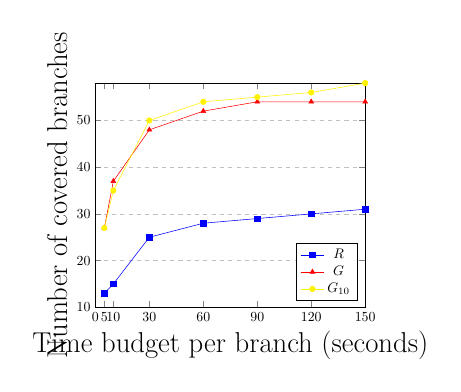
\begin{tikzpicture}[scale=0.5]
    \begin{axis}[
        xlabel={Time budget per branch (seconds)},
        ylabel={Number of covered branches},
        xmin=0, xmax=150,
        ymin=10, ymax=58,
        xtick={0,5,10,30,60,90,120,150,180},
        ytick={0,10,20,30,40,50},
        legend pos=south east,
        ymajorgrids=true,
        % xmajorgrids=true,
        grid style=dashed,
        label style={font=\huge}
      ]
      
      \addplot[
        color=blue,
        mark=square*,
      ] coordinates {
        (5,13) (10,15) (30,25) (60,28) (90,29) (120,30) (150,31)
      }; 
      \addplot[
        color=red,
        mark=triangle*,
      ]  coordinates {
        (5,27) (10,37) (30,48) (60,52) (90,54) (120,54) (150,54)
      };
      \addplot[
        color=yellow,
        mark=*,
      ]   coordinates {
        (5,27) (10,35) (30,50) (60,54) (90,55) (120,56) (150,58)
      };
      \legend{$\Random$,$\Genetic$,$\RGenetic$}
 
    \end{axis}
  \end{tikzpicture}
  \caption{Progress of the branch coverage given fix time budget per branch}
    \label{fig.budget.progress}
\end{figure}

Additionally, we would like to investigate how the coverage progresses with the increase of budget assigned per branch. This experiment models different testing scenarios, used in practice, which are time depended. E.g. running tests inside IDE should be fast; as part of the CI cycle we may afford a large waiting time; regression testing over night may take hours. Figure~\ref{fig.budget.progress} illustrates the progress of algorithms across various budget categories from 5 to 150 seconds per branch. Random test generation consistently underperforms the genetic one across all budget categories by at least factor of two. Eventually, it converges around 52\% coverage. Given 5 seconds per branch, both $\Genetic$ and $\RGenetic$ equally perform at the rate of 45\%. When the budget increases towards 10 seconds, $\Genetic$ slightly outperforms $\RGenetic$, 60\% against 63\% respectively. But when the budget rises to 30 seconds, $\RGenetic$ starts to transcend $\Genetic$ and the distance between them keeps growing further with the budget increase (starting from 120 seconds).\\ 
\setlength{\fboxsep}{1mm}
\fbox{%
  \parbox{8.2cm}{
Our recommendation is to use $\Genetic$ for rapid testing during development, and later in integration testing switch to $\RGenetic$ since it is able to reach harder to cover branches.
  }
}

\paragraph{\textbf{RQ2 (efficiency).}} To answer this question, we compare the actual execution time shown by our test algorithms in the experiments. Based on this information, we suggest an estimate on the execution time of the testing framework. The bar chart in Figure~\ref{fig.gen.time.comp} illustrates how the median coverage time varies for each algorithm at the function level. There are only two cases, \emph{revealAll} and \emph{doPaddlePower} out of 14, where $\Random$ just slightly outperformed $\RGenetic$ by 6\%, and two more cases \emph{shuffleBoard} and \emph{toggleInfo}, where they performed equally. In all other cases, $\RGenetic$ significantly outperformed $\Random$ by minimum 40\%~(\emph{newGame}) and maximum 510\%~(\emph{isValidCard}). 

\begin{figure}[t]
  \centering
  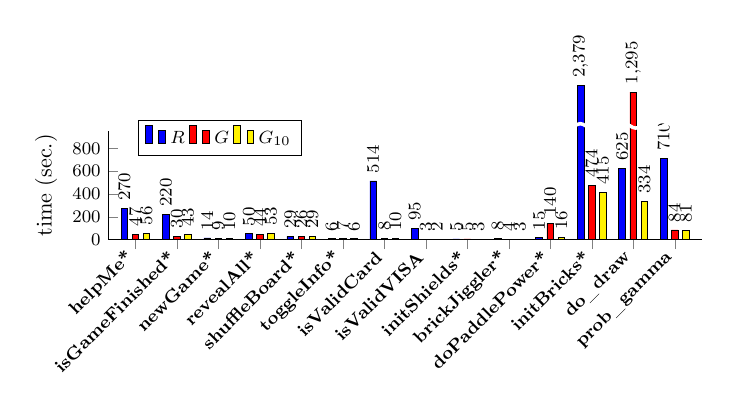
\begin{tikzpicture}[scale=0.8]
    \begin{axis}[
        every axis plot post/.style={/pgf/number format/fixed},
        ybar,
        ymin=0,ymax=950,
        width=11cm,height=3.3cm,
        bar width=3pt,
        enlarge x limits=0.05,
        legend style={at={(0.05,1.1)},anchor=north west,font=\footnotesize,legend columns=-1},
        legend cell align={left},
        ylabel={time (sec.)},
        symbolic x coords={helpMe*,isGameFinished*,newGame*,revealAll*,shuffleBoard*,toggleInfo*,isValidCard,isValidVISA,initShields*,brickJiggler*,doPaddlePower*,initBricks*,do\_draw,prob\_gamma},
        xtick=data,
        restrict y to domain*=0:1350, % Cut values off at 14
        visualization depends on=rawy\as\rawy, % Save the unclipped values
        after end axis/.code={ % Draw line indicating break
          \draw [ultra thick, white, decoration={snake, amplitude=1pt}, decorate] (rel axis cs:0,1.05) -- (rel axis cs:1,1.05);
        },
        nodes near coords={%
          \pgfmathprintnumber{\rawy}% Print unclipped values
        },
        every node near coord/.append style={rotate=90,anchor=west,font=\footnotesize},
        % every node near coord/.append style={font=\footnotesize},
        axis lines*=left,
        clip=false,
        x tick label style={rotate=45,anchor=east,font=\footnotesize\bfseries},
        y tick label style={font=\footnotesize}
      ]
      \addplot[fill=blue] coordinates {(helpMe*,270) (isGameFinished*,220) (newGame*,14) (revealAll*,50) (shuffleBoard*,29) (toggleInfo*,6) (isValidCard,514) (isValidVISA,95) (initShields*,5) (brickJiggler*,8) (doPaddlePower*,15)  (initBricks*,2379) (do\_draw,625) (prob\_gamma,710)};
      \addplot[fill=red] coordinates {(helpMe*,47)  (isGameFinished*,30)  (newGame*,9)  (revealAll*,44) (shuffleBoard*,26) (toggleInfo*,7) (isValidCard,8)   (isValidVISA,3)  (initShields*,5) (brickJiggler*,4) (doPaddlePower*,140) (initBricks*,474) (do\_draw,1295) (prob\_gamma,84)};
      \addplot[fill=yellow] coordinates {(helpMe*,56)  (isGameFinished*,43)  (newGame*,10) (revealAll*,53) (shuffleBoard*,29) (toggleInfo*,6) (isValidCard,10)  (isValidVISA,2)  (initShields*,3) (brickJiggler*,3) (doPaddlePower*,16) (initBricks*,415) (do\_draw,334) (prob\_gamma,81)}; 
      \legend{$\Random$,$\Genetic$,$\RGenetic$}
    \end{axis}
  \end{tikzpicture}
  \caption{Overall test generation time per function.}
  \label{fig.gen.time.comp}
\end{figure}  

%% \begin{figure}[t]
%%   \begin{tikzpicture}[scale=0.8]
%%     \begin{axis}[
%%         every axis plot post/.style={/pgf/number format/fixed},
%%         ybar,
%%         ymin=0,ymax=135,
%%         width=11cm,height=3.3cm,
%%         bar width=3pt,
%%         enlarge x limits=0.05,
%%         legend style={at={(0.05,1.2)},anchor=north west,font=\footnotesize,legend columns=-1},
%%         legend cell align={left},
%%         ylabel={time (sec.)},
%%         symbolic x coords={helpMe*,isGameFinished*,newGame*,revealAll*,shuffleBoard*,toggleInfo*,isValidCard,isValidVISA,initShields*,brickJiggler*,doPaddlePower*,initBricks*,do\_draw,prob\_gamma},
%%         xtick=data,
%%         nodes near coords,
%%         every node near coord/.append style={rotate=90, anchor=west, font=\footnotesize},
%%         % every node near coord/.append style={font=\footnotesize},
%%         axis lines*=left,
%%         clip=false,
%%         x tick label style={rotate=45,anchor=east,font=\footnotesize\bfseries},
%%         y tick label style={font=\footnotesize}
%%       ]
%%       \addplot[fill=blue] coordinates {(helpMe*,54) (isGameFinished*,44) (newGame*,4.7) (revealAll*,25) (shuffleBoard*,3.6) (toggleInfo*,1.5) (isValidCard,85.7) (isValidVISA,47.5) (initShields*,5) (brickJiggler*,4) (doPaddlePower*,3.75)  (initBricks*,132.16) (do\_draw,28.5) (prob\_gamma,44.4)};
      
%%       \addplot[fill=red] coordinates {(helpMe*,9.4)  (isGameFinished*,6)  (newGame*,3)  (revealAll*,22) (shuffleBoard*,3.25) (toggleInfo*,1.75) (isValidCard,1.33)   (isValidVISA,1.5)  (initShields*,4) (brickJiggler*,2) (doPaddlePower*,35) (initBricks*,26.33) (do\_draw,58.9) (prob\_gamma,5.25)};
      
%%       \addplot[fill=yellow] coordinates {(helpMe*,11.2)  (isGameFinished*,8.6)  (newGame*,3.3) (revealAll*,26.5) (shuffleBoard*,3.6) (toggleInfo*,1.5) (isValidCard,1.66)  (isValidVISA,1)  (initShields*,3) (brickJiggler*,1.5) (doPaddlePower*,4) (initBricks*,23.1) (do\_draw,15.18) (prob\_gamma,5.1)}; 
%%       \legend{$\Random$,$\Genetic$,$\RGenetic$}
%%     \end{axis}
%%   \end{tikzpicture}
%%   \caption{Average generation time per branch}
%%     \label{fig.gen.time.branch}
%% \end{figure}

Looking separately at the average execution time for \emph{simple} and \emph{difficult} functions in Table~\ref{tbl.stats.sum}, we conclude that $\RGenetic$ was the fastest algorithm in both cases with the 7 and 25 seconds per branch. For simple functions, the $\Genetic$'s performance was quite close to $\RGenetic$, only 9 seconds, but was two times slower for difficult functions. In all categories, $\Random$ was much slower than both genetic alternatives.\\
\setlength{\fboxsep}{1mm}
\fbox{%
  \parbox{8.2cm}{
    Globally, $\RGenetic$ outperformed both $\Genetic$ and $\Random$ with an average execution time per branch 19, 39 and 88 seconds, respectively. 
  }
}

\begin{figure}[t]
  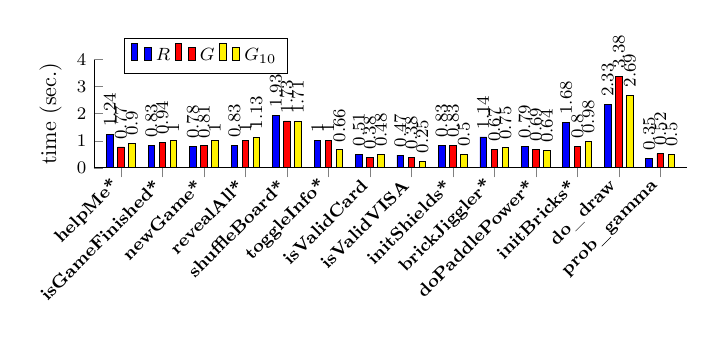
\begin{tikzpicture}[scale=0.8]
    \begin{axis}[
        every axis plot post/.style={/pgf/number format/fixed},
        ybar,
        ymin=0,ymax=4,
        width=11cm,height=3.3cm,
        bar width=3pt,
        enlarge x limits=0.05,
        legend style={at={(0.05,1.2)},anchor=north west,font=\footnotesize,legend columns=-1},
        legend cell align={left},
        ylabel={time (sec.)},
        symbolic x coords={helpMe*,isGameFinished*,newGame*,revealAll*,shuffleBoard*,toggleInfo*,isValidCard,isValidVISA,initShields*,brickJiggler*,doPaddlePower*,initBricks*,do\_draw,prob\_gamma},
        xtick=data,
        nodes near coords,
        every node near coord/.append style={rotate=90, anchor=west, font=\footnotesize},
        % every node near coord/.append style={font=\footnotesize},
        axis lines*=left,
        clip=false,
        x tick label style={rotate=45,anchor=east,font=\footnotesize\bfseries},
        y tick label style={font=\footnotesize}
      ]
      \addplot[fill=blue] coordinates {(helpMe*,1.24) (isGameFinished*,0.83) (newGame*,0.78) (revealAll*,0.83) (shuffleBoard*,1.93) (toggleInfo*,1) (isValidCard,0.51) (isValidVISA,0.47) (initShields*,0.83) (brickJiggler*,1.14) (doPaddlePower*,0.79)  (initBricks*,1.68) (do\_draw,2.33) (prob\_gamma,0.35)};
      \addplot[fill=red] coordinates {(helpMe*,0.77)  (isGameFinished*,0.94)  (newGame*,0.81)  (revealAll*,1) (shuffleBoard*,1.73) (toggleInfo*,1) (isValidCard,0.38)   (isValidVISA,0.38)  (initShields*,0.83) (brickJiggler*,0.67) (doPaddlePower*,0.69) (initBricks*,0.8) (do\_draw,3.38) (prob\_gamma,0.52)};
      \addplot[fill=yellow] coordinates {(helpMe*,0.9)  (isGameFinished*,1)  (newGame*,1) (revealAll*,1.13) (shuffleBoard*,1.71) (toggleInfo*,0.66) (isValidCard,0.48)  (isValidVISA,0.25)  (initShields*,0.5) (brickJiggler*,0.75) (doPaddlePower*,0.64) (initBricks*,0.98) (do\_draw,2.69) (prob\_gamma,0.5)}; 
      \legend{$\Random$,$\Genetic$,$\RGenetic$}
    \end{axis}
  \end{tikzpicture}
  \caption{Speed of test generation measured as $t/i$}
    \label{fig.get.cost}
\end{figure}

Another question, related to the efficiency of our framework, is the computational cost of one iteration of the algorithm. This information is useful when configuring the maximal generation limit. The cost, shown in column $t/i$ in Table~\ref{tbl.stats}, is calculated as the relation between the execution time and the number of generations, i.e. it measures the speed of one iteration. Figure~\ref{fig.get.cost} presents the cost comparison of three algorithms across all functions in our study. On the one hand, the cost of one iteration depends on the population size, 50 candidates in our case. On the other hand, it also depends on the length of the execution trace produced during the evaluation of a candidate, because longer traces increase the computation cost the fitness function.  Premature program termination due to exceptions leads to short traces, whereas loops and program size in the general contribute to the longer traces. For example, the \emph{do_draw} function produces long traces because it only operates with the primitive types thus not rising exceptions, and at the same time, it consists of 40 LOC. In our evaluation we observed that the iteration cost varied between 0.25 and 3.59 seconds.\\
\setlength{\fboxsep}{1mm}
\fbox{%
  \parbox{8.2cm}{
    Globally, one algorithm iteration took one second for $\Random$ and $\RGenetic$, with $\Genetic$ performing worse 1.4 seconds.
  }
} 
  

\paragraph{\textbf{RQ3 (significance).}} Because our testing framework is randomized by nature, we need to conduct statistical analysis to test the \emph{significance} and \emph{effect size} of our the performance results. This analysis is based on the coverage time in 50 executions, produced by each test algorithm $\Random$, $\Genetic$ and $\RGenetic$. Following recommendations on the assessment of randomized algorithms~\cite{arcuri2011practical}, we use the non-parametric Mann-Whitney U-test~\cite{mann1947test} and the Vargha-Delaney $\hat{A}_{12}$ statistics~\cite{vargha2000critique} for measuring statistical significance ($\alpha=0.05$) and effect size, respectively. In Table~\ref{tbl.stats} the three columns to the right show the $\hat{A}_{12}$ values for all algorithm combinations, where this value is significant and '-' otherwise. For example, the higher the value in the $_{\Genetic}^{\Random}$ column, the slower $\Random$ performs comparing to $\Genetic$. Depends on the actual $\hat{A}_{12}$ value, the effect size can be small (0.56), medium (0.64), and large (0.71).\\
\setlength{\fboxsep}{1mm}
\fbox{%
  \parbox{8.2cm}{
    Both $\Genetic$ and $\RGenetic$ largely outperform $\Random$ in 50\% cases globally and 67\% on the difficult functions.  
  }
}  


% % \setlength\tabcolsep{0.5pt}
\begin{table*}
  \caption{Statistics for genetic and random algorithms}
  \label{tbl.stats}
  \resizebox{\textwidth}{!}{
    \large
    \begin{tabular}{l|rrrr|rrrr|rrrr|rrrr|r|r|r|r|r|r}
      \toprule
      \textbf{name}   & $\bar{x}_R$     & $\bar{x}_G$   & $\bar{x}_{G5}$ & $\bar{x}_{G10}$ & $m_R$       & $m_G$     & $m_{G5}$     & $m_{G10}$   & $\min_R$  & $\min_G$ & $\min_{G5}$ & $\min_{G10}$ & $\max_R$  & $\max_G$ & $\max_{G5}$ & $\max_{G10}$ & \textbf{R-G} & \textbf{R-G5} & \textbf{R-G10} & \textbf{G-5} & \textbf{G-G10} & \textbf{G5-G10}\\
      \toprule
      helpMe          & 235.68 / 293    & 74.04 / 63.18 & 83.66 / 78.34 & 84.34 / 80.68 & 211.5 / 270 & 55.5 / 47   & 62   / 59.5 & 56.5 / 55.5 & 25 / 33   & 8 / 7    & 8 / 8      & 10 / 12     & 445 / 609 & 286 / 258 & 401 / 368  & 494 / 468 & & & & & & \\
    $(3,4,\inFor)$    & 3.94   / 5.34   & 7.94  / 6.24  & 10.22 / 8.48  & 11.7  / 9.32  & 3     / 4   & 3.5  / 3    & 7    / 6    & 7    / 6    & 1 / 1     & 1 / 1    & 1 / 1      & 1 / 2       & 16 / 21   & 31 / 23   & 63 / 48    & 124 / 84  & 0.45 / 0.57 & 0.32 / 0.41 & 0.29 / 0.39 & 0.41 / 0.38 & 0.39 / 0.37 & 0.47 / 0.47 \\
    $(5,6,\thenBr)$   & 3.7    / 5.74   & 13.08 / 9.86  &   9.2 / 7.76  & 9.6   / 8.06  & 3     / 5   & 7    / 5.5  & 5    / 4    & 5.5  / 5    & 1 / 2     & 1 / 1    & 1 / 1      & 1 / 1       & 14 / 28   & 95 / 68   & 44 / 38    & 105 / 89  & 0.32 / 0.46 & 0.32 / 0.47 & 0.36 / 0.5  & 0.54 / 0.52 & 0.55 / 0.53 & 0.52 / 0.52 \\
    $(5,15,\elseBr)$  & 118.64 / 151.48 & 30.14 / 27.08 & 34.12 / 32.7  & 31.68 / 31.92 & 119.5 / 156 & 23   / 20.5 & 28.5 / 28.5 & 22   / 23.5 & 4 / 6     & 4 / 3    & 3 / 3      & 1 / 2       & 199 / 294 & 97 / 99   & 167 / 156  & 114 / 130 & 0.83 / 0.87 & 0.81 / 0.85 & 0.83 / 0.86 & 0.45 / 0.42 & 0.52 / 0.48 & 0.56 / 0.55 \\
    $(9,10,\thenBr)$  & 105.12 / 124.26 & 17.82 / 15.58 & 21.98 / 21.66 & 21.8  / 21.9  & 83.5  / 101 & 17   / 14   & 17.5 / 17   & 18   / 17   & 18 / 23   & 1 / 1    & 2 / 2      & 6 / 6       & 199 / 245 & 53 / 51   & 78 / 83    & 77  / 86  & 0.96 / 0.98 & 0.93 / 0.95 & 0.93 / 0.95 & 0.46 / 0.43 & 0.45 / 0.40 & 0.49 / 0.47 \\
    $(9,14,\elseBr$   & 4.28   / 6.18   & 5.06  / 4.42  &  8.14 / 7.74  & 9.56  / 9.48  & 2.5   / 4   & 5    / 4    & 4    / 4    & 4    / 4    & 1 / 1     & 1 / 1    & 1 / 1      & 1 / 1       & 17 / 21   & 20 / 17   & 49 / 43    & 74  / 79  & 0.39 / 0.56 & 0.43 / 0.53 & 0.39 / 0.51 & 0.53 / 0.48 & 0.49 / 0.45 & 0.46 / 0.48 \\
    \midrule
    isGameFinished      & 343.82 / 290.26 & 132.76 / 135.06 & 69.32 / 75.68 & 71.12 / 77.48 & 258 / 219.5 & 27 / 30   & 34.5 / 39   & 38 / 43   & 200 / 142 & 1 / 2   &  1 / 3    & 2 / 5       & 598 / 573 & 601 / 668 & 600 / 676  & 484 / 513 &             &              &             &             &             &      \\
    %% $(5,6,\inFor)$   & 0.02 / 0        & 0.1 / 0.88      & 0.12 / 0.94   & 0.1 / 0.94    & 0 / 1       & 0 / 1     & 0 / 1       & 0 / 1     & 0 / 0     & 0 / 0   & 0 / 0     & 0 / 0       & 1 / 2     & 2 / 3     & 2 / 3      & 2 / 3     & 0.47 / 0.53 & 0.46 / 0.5   & 0.47 / 0.5  & 0.49 / 0.48 & 0.5 / 0.47  & 0.51 / 0.5 \\
    $(7,8,\thenBr)$     & 75.18 / 63.68   & 40.54 / 40.32   & 18.86 / 19.62 & 14.66 / 15.62 & 35.5 / 29.5 & 7 / 7.5   & 8 / 9.5     & 11 / 12.5 & 0 / 0     & 0 / 0   & 0 / 1     & 0 / 1       & 199 / 191 & 199 / 225 & 199 / 196  & 82 / 77   & 0.64 / 0.6  & 0.7 / 0.66   & 0.69 / 0.66 & 0.48 / 0.46 & 0.45 / 0.43 & 0.43 / 0.44  \\
    %% $(7,15,\elseBr)$ & 0 / 0.98        & 0.06 / 0.82     & 0.04 / 0.84   & 0.08 / 0.9    & 0 / 1       & 0 / 1     & 0 / 1       & 0 / 1     & 0 / 0     & 0 / 0   & 0 / 0     & 0 / 0       & 0 / 3     & 2 / 3     & 1 / 2      & 2 / 3     & 0.48 / 0.57 & 0.48 / 0.55  & 0.47 / 0.54 & 0.5 / 0.48  & 0.49 / 0.46 & 0.49 / 0.48 \\
    $(10,11,\thenBr)$   & 199 / 166.32    & 35.74 / 36.6    & 21.56 / 22.5  & 24.36 / 26.44 & 199 / 167   & 10 / 10   & 10 / 10.5   & 9 / 11    & 199 / 141 & 1 / 2   & 1 / 1     & 2 / 3       & 199 / 191 & 199 / 220 & 199 / 217  & 199 / 224 & 0.94 / 0.88 & 0.98 / 0.96  & 0.98 / 0.96 & 0.53 / 0.52 & 0.52 / 0.48 & 0.47 / 0.45 \\
    $(10,14,\elseBr)$   & 69.62 / 59.28   & 56.32 / 56.44   & 28.74 / 31.78 & 31.92 / 33.58 & 23.5 / 21   & 10 / 10.5 & 16.5 / 17   & 18 / 17.5 & 1 / 1     & 0 / 0   & 0 / 1     & 0 / 1       & 199 / 186 & 199 / 217 & 199 / 258  & 199 / 206 & 0.6 / 0.55  & 0.611 / 0.57 & 0.6 / 0.55  & 0.5 / 0.48  & 0.48 / 0.46 & 0.47 / 0.47 \\
    \midrule
    newGame             & 21.64 / 18.26 & 10.74 / 11.28 & 10.12 / 11.94  & 8.38 / 10.5   & 15 / 13.5   & 7.5 / 9   & 7.5 / 10    & 7 / 10   & 0 / 1      & 0 / 1    & 0 / 1      & 0 / 0       & 99 / 69  & 58 / 53    & 33 / 39    & 36 / 34 & & & & & & \\
    %% $(4,5,\inFor)$   & 0.04 / 0.9    & 0.12 / 0.66   & 0.1 / 0.84     & 0 / 0.86      & 0 / 1       & 0 / 1     & 0 / 1       & 0 / 1     & 0 / 0     & 0 / 0    & 0 / 0      & 0 / 0       & 1 / 2    & 2 / 2      & 1 / 2      & 0 / 1   & 0.47 / 0.6  & 0.47 / 0.53 & 0.52 / 0.51 & 0.5 / 0.42  & 0.54 / 0.4 & 0.55 / 0.49 \\
    $(6,7,\thenBr)$     & 21.54 / 16.58 & 10.48 / 9.78  & 9.92 / 10.24   & 8.34 / 8.84   & 15 / 11.5   & 7.5 / 7   & 7.5 / 8     & 7 / 8     & 0 / 1     & 0 / 1    & 0 / 1      & 0 / 0       & 97 / 67  & 53 / 47    & 30 / 34    & 35 / 31 & 0.68 / 0.64 & 0.67 / 0.6  & 0.72 / 0.65 & 0.48 / 0.44 & 0.55 / 0.5 & 0.56 / 0.56 \\
    %% $(6,12,\elseBr)$ & 0.06 / 0.78   & 0.14 / 0.84   & 0.1 / 0.86     & 0.04 / 0.8    & 0 / 1       & 0 / 1     & 0 / 1       & 0 / 1     & 0 / 0     & 0 / 0    & 0 / 0      & 0 / 0       & 1 / 2    & 3 / 4      & 2 / 3      & 1 / 2   & 0.5 / 0.5   & 0.49 / 0.47 & 0.51 / 0.49 & 0.49 / 0.46 & 0.5 / 0.48 & 0.52 / 0.52 \\
    \midrule
    revealAll           & 77.9 / 69.2   & 51.06 / 55.26 & 65.04 / 70.34 & 55.68 / 64.04 & 58 / 50     & 42 / 44   & 55.5 / 58.5 & 44.5 / 52.5 & 9 / 8     & 16 / 16  & 16 / 16    & 16 / 16     & 305 / 261 & 135 / 153  & 200 / 226  & 165 / 202 & & & & & &\\
    $(2,3,\inFor)$      & 31.78 / 27.78 & 24.84 / 26.7  & 34.94 / 39.34 & 28.04 / 32.58 & 24 / 20     & 23 / 24   & 29 / 30.5   & 22.5 / 27   & 4 / 3     & 7 / 7    & 7 / 7      & 10 / 11     & 106 / 89  & 57 / 64    & 129 / 148  & 75 / 100  & 0.53 / 0.45 & 0.44 / 0.37 & 0.49 / 0.39 & 0.39 / 0.39 & 0.46 / 0.43 & 0.57 / 0.55 \\
    $(4,5,\inFor)$      & 46.12 / 41.42 & 26.22 / 28.56 & 30.1 / 33.02  & 27.64 / 31.46 & 34 / 30     & 19 / 20   & 26.5 / 28   & 22 / 25.5   & 5 / 5     & 9 / 9    & 9 / 9      & 6 / 5       & 199 / 172 & 78 / 89    & 71 / 78    & 90 / 102  & 0.68 / 0.62 & 0.6 / 0.53  & 0.65 / 0.55 & 0.4 / 0.39  & 0.41 / 0.37 & 0.55 / 0.53 \\
    \midrule
    shuffleBoard         & 211.4 / 410.56 & 218.88 / 321.28 & 224.92 / 371.58 & 222.26 / 358.84 & 206.5 / 401.5 & 207 / 299   & 212.5 / 338 & 209 / 321 & 199 / 342 & 199 / 250 & 199 / 268 & 199 / 263 & 258 / 568 & 402 / 689 & 351 / 716 & 360 / 674 & & & & & & \\
    %% $(3,4,\inFor)$    & 0 / 1.6        & 0 / 1.36        & 0 / 1.52        & 0 / 1.42        & 0 / 2         & 0 / 1       & 0 / 2       & 0 / 1     & 0 / 1     & 0 / 1     & 0 / 1     & 0 / 1     & 0 / 3     & 0 / 2     & 0 / 2     & 0 / 2     & 0.5 / 0.61  & 0.5 / 0.54  & 0.5 / 0.58  & 0.5 / 0.42  & 0.5 / 0.47  & 0.5 / 0.55 \\
    %% $(5,6,\inWhile)$  & 0.36 / 2.94    & 0.32 / 2.6      & 0.24 / 2.58     & 0.38 / 2.88     & 0 / 2         & 0 / 2       & 0 / 2       & 0 / 2     & 0 / 1     & 0 / 1     & 0 / 1     & 0 / 1     & 4 / 11    & 3 / 8     & 2 / 6     & 5 / 15    & 0.52 / 0.6  & 0.51 / 0.54 & 0.52 / 0.56 & 0.5 / 0.45  & 0.5 / 0.46  & 0.5 / 0.52 \\
    %% $(10,11,\inFor)$  & 0 / 1.88       & 0 / 1.4         & 0 / 1.64        & 0 / 1.58        & 0 / 2         & 0 / 1       & 0 / 2       & 0 / 2     & 0 / 2     & 0 / 1     & 0 / 1     & 0 / 1     & 0 / 3     & 0 / 2     & 0 / 2     & 0 / 2     & 0.5 / 0.72  & 0.5 / 0.61  & 0.5 / 0.64  & 0.5 / 0.38  & 0.5 / 0.41  & 0.5 / 0.53 \\
    $(13,14,\thenBr)$    & 6.38 / 13.6    & 7.7 / 13.88     & 8.72 / 17.7     & 7.86 / 15.78    & 4 / 9.5       & 4 / 8.5     & 4 / 8.5     & 5 / 9.5   & 0 / 1     & 0 / 1     & 0 / 1     & 0 / 1     & 22 / 44   & 67 / 103  & 64 / 126  & 38 / 78   & 0.54 / 0.58 & 0.5 / 0.52  & 0.5 / 0.53  & 0.46 / 0.46 & 0.47 / 0.46 & 0.52 / 0.51 \\
    % $(13,16,\elseBr)$  & 0 / 1.52       & 0 / 1.4         & 0 / 1.68        & 0 / 1.5         & 0 / 1.5       & 0 / 1       & 0 / 2       & 0 / 1.5   & 0 / 1     & 0 / 1     & 0 / 1     & 0 / 1     & 0 / 3     & 0 / 2     & 0 / 2     & 0 / 2     & 0.5 / 0.55  & 0.5 / 0.42  & 0.5 / 0.51  & 0.5 / 0.36  & 0.5 / 0.45  & 0.5 / 0.59 \\
    $(17,18,\thenBr)$    & 5.66 / 13.76   & 11.86 / 23.7    & 16.96 / 39.58   & 15.02 / 34.04   & 3.5 / 10      & 4 / 10      & 5.5 / 12.5  & 5 / 1     & 0 / 1     & 0 / 2     & 0 / 2     & 0 / 2     & 33 / 73   & 133 / 248 & 86 / 180  & 118 / 248 & 0.43 / 0.46 & 0.37 / 0.38 & 0.45 / 0.47 & 0.43 / 0.4  & 0.5 / 0.5   & 0.55 / 0.55 \\
    %% $(17,20,\elseBr)$ & 0 / 2.06       & 0 / 1.84        & 0 / 1.72        & 0 / 1.8         & 0 / 2         & 0 / 2       & 0 / 2       & 0 / 2     & 0 / 1     & 0 / 1     & 0 / 1     & 0 / 1     &  0 / 4    & 0 / 2     & 0 / 2     & 0 / 2     & 0.5 / 0.59  & 0.5 / 0.64  & 0.5 / 0.61  & 0.5 / 0.56  & 0.5 / 0.52  & 0.5 / 0.46 \\
    $(21,22,\inFor)$     & 199 / 373.2    & 199 / 275.1     & 199 / 305.16    & 199 / 299.84    & 199 / 372.5   & 199 / 273.5 & 199 / 307   & 199 / 302 & 199 / 334 & 199 / 242 & 199 / 260 & 199 / 255 & 199 / 427 & 199 / 322 & 199 / 396 & 199 / 325 & 0.5 / 1     & 0.5 / 0.99  & 0.5 / 1     & 0.5 / 0.15 & 0.5 / 0.16   & 0.5 / 0.58 \\
    \midrule
    \midrule
    toggleInfo         & 3.06 / 6.12 & 11.02 / 11.9 & 18.1 / 18.3 & 16.3 / 15.4  & 2 / 5.5 & 3 / 7 & 5  7.5  & 5 / 6 & 0 / 0 & 0 / 0 & 0 / 0 & 0 / 0 & 19 / 22 & 129 / 118 & 146 / 138 & 139 / 106 & & & & & & \\
    $(2,3,\thenBr)$    & 1.58 / 2.32 & 1.12 / 1.64  & 1.1 / 1.7   & 1 / 1.46     & 1 / 1.5 & 1 / 2 & 1 / 2   & 1 / 1 & 0 / 0 & 0 / 0 & 0 / 0 & 0 / 0 & 11 / 11 & 4 / 4     & 3 / 4     & 3 / 3     & 0.5 / 0.54  & 0.51 / 0.53 & 0.53 / 0.58 & 0.5 / 0.48  & 0.53 / 0.55 & 0.53 / 0.57 \\
    %% $(2,5,\elseBr)$ & 0 / 0.86    & 0 / 0.84     & 0 / 0.86    & 0 / 0.8      & 0 / 1   & 0 / 1 & 0 / 1   & 0 / 1 & 0 / 0 & 0 / 0 & 0 / 0 & 0 / 0 & 0 / 2   & 0 / 1     & 0 / 1     & 0 / 1     & 0.5 / 0.51  & 0.5 / 0.5   & 0.5 / 0.53  & 0.5 / 0.49  & 0.5 / 0.52  & 0s.5 / 0.53 \\
    $(6,7,\thenBr)$    & 1.48 / 2.1  & 9.9 / 8.7    & 17 / 14.92  & 15.3 / 12.34 & 1 / 2   & 2 / 3 & 4 / 3.5 & 4 / 3 & 0 / 0 & 0 / 0 & 0 / 0 & 0 / 0 & 8 / 8   & 125 / 112 & 143 / 132 & 136 / 101 & 0.36 / 0.37 & 0.28 / 0.29 & 0.34 / 0.36 & 0.43 / 0.42 & 0.48 / 0.48 & 0.53 / 0.55 \\
    %% $(6,13,\elseBr)$& 0 / 0.84    & 0 / 0.72     &  0 / 0.82   & 0 / 0.8      & 0 / 1   & 0 / 1 & 0 / 1   & 0 / 1 & 0 / 0 & 0 / 0 & 0 / 0 & 0 / 0 & 0 / 1   & 0 / 1     & 0 / 1     & 0 / 1     & 0.5 / 0.56  & 0.5 / 0.51  & 0.5 / 0.52  & 0.5 / 0.45  & 0.5 / 0.46  & 0.5 / 0.51 \\
    \midrule
    \midrule
    isValidCard       & 995 / 513.66 & 14.76 / 7.8 & 14.8 / 7.96 & 14.82 / 8.42 & 995 / 514   & 15 / 8 & 15 / 7 & 15 / 9.5 & 995 / 447 & 10 / 5 & 10 / 5 & 10 / 5 & 995 / 579 & 22 / 12 & 24 / 13 & 24 / 12  & & & & & & \\
    %% $(3,4,\thenBr)$   & 0 / 0.54     & 0 / 0.3     & 0 / 0.46    & 0 / 0.46     & 0 / 1       & 0 / 0  & 0 / 0  & 0 / 0    & 0 / 0     & 0 / 0  & 0 / 0  & 0 / 0  & 0 / 0     & 0 / 1   & 0 / 1   & 0 / 0 & 0.5 / 0.61 & 0.5 / 0.53 & 0.5 / 0.53 & 0.5 / 0.42 & 0.5 / 0.42 & 0.5 / 0.5 \\
    $(3,6,\elseBr)$   & 199 / 102.98 & 2.98 / 1.52 & 3 / 1.4     & 2.82 / 1.56  & 199 / 102.5 & 3 / 2  & 3 / 1  & 3 / 2    & 199 / 87  & 2 / 1  & 2 / 1  & 2 / 1  & 199 / 116 & 5 / 2   & 5 / 3   & 4 / 3    & 1 / 1 & 1 / 1 & 1 / 1 & 0 / 0.49    & 0.55 / 0.5  & 0.56 / 0.43 \\
    $(7,8,\inFor)$    & 199 / 102.38 & 2.92 / 1.44 & 3.04 / 1.6  & 2.96 / 1.58  & 199 / 103   & 3 / 1  & 3 / 2  & 3 / 2    & 199 / 90  & 2 / 1  & 2 / 1  & 2 / 1  & 199 / 115 & 5 / 3   & 4 / 2   & 5 / 2    & 1 / 1 & 1 / 1 & 1 / 1 & 0.45 / 0.42 & 0.48 / 0.43 & 0.53 / 0.51 \\
    $(10,11,\thenBr)$ & 199 / 101.44 & 3 / 1.56    & 2.86 / 1.48 & 3.06 / 1.7   & 199 / 102   & 3 / 2  & 3 / 1  & 3 / 2    & 199 / 88  & 2 / 1  & 2 / 1  & 2 / 1  & 199 / 116 & 4 / 2   & 5 / 2   & 5 / 3    & 1 / 1 & 1 / 1 & 1 / 1 & 0.55 / 0.54 & 0.48 / 0.43 & 0.43 / 0.4 \\
    $(10,13,\elseBr)$ & 199 / 104.66 & 2.84 / 1.38 & 2.98 / 1.54 & 3.04 / 1.62  & 199 / 106   & 3 / 1  & 3 / 2  & 3 / 2    & 199 / 91  & 2 / 1  & 2 / 1  & 2 / 1  & 199 / 115 & 4 / 2   & 5 / 2   & 5 / 2    & 1 / 1 & 1 / 1 & 1 / 1 & 0.46 / 0.42 & 0.42 / 0.38 & 0.48 / 0.46 \\
    $(14,15,\inFor)$  & 199 / 101.66 & 3.02 / 1.6  & 2.92 / 1.48 & 2.94 / 1.5   & 199 / 99.5  & 3 / 2  & 3 / 1  & 3 / 1.5  & 199 / 91  & 2 / 1  & 2 / 1  & 2 / 1  & 199 / 117 & 4 / 2   & 5 / 3   & 5 / 2    & 1 / 1 & 1 / 1 & 1 / 1 & 0.55 / 0.56 & 0.54 / 0.55 & 0.48 / 0.48 \\
    \midrule
    isValidMasterCard  & 199 / 109.46 & 11.04 / 4.84 & 12.08 / 5.1  & 11.42 / 5.03 & 199 / 102.5 & 10 / 4 & 12 / 4.5 & 10 / 4 & 199 / 86 & 4 / 2 & 5 / 2 & 5 / 2 & 199 / 164 & 27 / 11 & 32 / 11 & 23 / 10 & & & & & & \\
    $(2,3,\thenBr)$    & 199 / 108.98 & 11.04 / 4.5  & 12.08 / 4.64 & 11.42 / 4.6  & 199 / 102.5 & 10 / 4 & 12 / 4.5 & 10 / 4 & 199 / 86 & 4 / 2 & 5 / 2 & 5 / 2 & 199 / 162 & 27 / 10 & 32 / 10 & 23 / 9  & 1 / 1      & 1 / 1     & 1 / 1 & 0.43 / 0.47 & 0.47 / 0.49 & 0.53 / 0.51 \\
    %% $(2,5,\elseBr)$ & 0 / 0.48     & 0 / 0.34     & 0 / 0.46     & 0 / 0.43     & 0 / 0       & 0 / 0  & 0 / 0    & 0 / 0  & 0 / 0    & 0 / 0 & 0 / 0 & 0 / 0 & 0 / 2     & 0 / 1   & 0 / 1   & 0 / 1   & 0.5 / 0.56 & 0.5 / 0.5 & 0.5 / 0.52 & 0.5 / 0.44 & 0.5 / 0.46 & 0.5 / 0.52 \\
    \midrule
    isValidVISA       & 199 / 97.54 & 6.54 / 3.06 & 6.38 / 3.04 & 6.48 / 3.04 & 199 / 95 & 6 / 3 & 6 / 3 & 6 / 2 & 199 / 89 & 4 /2  & 3 / 1 & 4 / 1 & 199 / 140 & 14 / 6 & 16 / 7 & 18 / 7 & & & & & & \\
    $(2,3,\thenBr)$   & 199 / 97.08 & 6.54 / 2.72 & 6.38 / 2.62 & 6.48 / 2.58 & 199 / 95 & 6 / 3 & 6 / 3 & 6 / 2 & 199 / 89 & 4 / 2 & 3 / 1 & 4 / 1 & 199 / 139 & 14 / 5 & 16 / 6 & 18 / 6 & 1 / 1 & 1 / 1 & 1 / 1 & 0.57 / 0.54 & 0.55 / 0.59 & 0.48 / 0.54 \\
    %% $(2,5,\elseBr)$   & 0 / 0.46    & 0 / 0.34    & 0 / 0.42    & 0 / 0.46    & 0 / 0    & 0 / 0 & 0 / 0 & 0 / 0 & 0 / 0    & 0 / 0 & 0 / 0 & 0 / 0 & 0 / 1     & 0 / 1  & 0 / 1  & 0 / 1  & 0.5 / 0.56 & 0.5 / 0.52 & 0.5 / 0.5 & 0.5 / 0.46 & 0.5 / 0.44 & 0.5 / 0.48 \\
    \midrule
    \midrule
    initShields       & 5 / 5.8 & 5.32 / 3.76 & 5.28 / 3.9 & 5.26 / 3.7 & 5 / 5 & 5 / 4 & 5 / 4 & 5 / 3 & 5 / 3 & 5 / 3 & 5 / 3 & 5 / 3 & 5 / 10 & 6 / 5 & 7 / 5 & 7 / 5 & & & & & & \\
    $(2,3,\inFor)$    & 5 / 5.8 & 5.32 / 3.76 & 5.28 / 3.9 & 5.26 / 3.7 & 5 / 5 & 5 / 4 & 5 / 4 & 5 / 3 & 5 / 3 & 5 / 3 & 5 / 3 & 5 / 3 & 5 / 10 & 6 / 5 & 7 / 5 & 7 / 5 & 0.34 / 0.83 & 0.37 / 0.8 & 0.38 / 0.84 & 0.53 / 0.45 & 0.54 / 0.53 & 0.51 / 0.58 \\
    \midrule
    \midrule
    brickJiggler      & 5.22 / 9.74 & 5.34 / 4.68 & 5.68 / 4.98 & 5.3 / 4.28 & 5 / 8 & 4 / 4 & 8 / 4 & 2 / 3 & 1 / 2 & 2 / 3 & 1 / 2 & 1 / 2 & 18 / 28 & 39 / 20 & 20 / 12 & 20 / 12 &  & & & & &\\
    $(2,3,\thenBr)$   & 5.22 / 8.46 & 5.34 / 3.54 & 5.68 / 3.66 & 5.3 / 3.2  & 5 / 7 & 4 / 3 & 4 / 3 & 2 / 2 & 1 / 2 & 2 / 2 & 1 / 1 & 1 / 1 & 18 / 25 & 39 / 18 & 20 / 10 & 20 / 10 & 0.54 / 0.83 & 0.51 / 0.81 & 0.54 / 0.85 & 0.49 / 0.48 & 0.5 / 0.56 & 0.52 / 0.57 \\
    %% $(2,9,\elseBr)$& 0 / 1.28    & 0 / 1.14    & 0 / 1.32    & 0 / 1.08   & 0 / 1 & 0 / 1 & 4 / 1 & 0 / 1 & 0 / 0 & 0 / 1 & 0 / 1 & 0 / 1 & 0 / 3   & 0 / 2   & 0 / 2   & 0 / 2   & 0.5 / 0.51  & 0.5 / 0.45  & 0.5 / 0.53  & 0.5 / 0.41  & 0.5 / 0.53 & 0.5 / 0.62 \\
    \midrule
    doPaddlePower        & 18.1 / 17.64  & 193.54 / 134.54 & 47.32 / 36.4  & 42.78 / 29.58 & 14.5 / 15 & 199 / 140 & 17 / 14 & 21 / 16 & 1 / 1 & 3 / 3 & 0 / 0 & 0 / 1 & 54 / 51 & 204 / 160 & 202 / 157 & 204 / 144 & & & & & & \\
    %% $(5,6,\thenBr)$   & 0 / 0.82      & 0 / 0.82        & 0 / 0.9       & 0 / 0.86      & 0 / 1     & 0 / 1     & 0 / 1   & 0 / 1   & 0 / 0 & 0 / 0 & 0 / 0 & 0 0   & 0 / 2   & 0 / 1     & 0 / 1     & 0 / 1     & 0.5 / 0.5   & 0.5 / 0.46  & 0.5 / 0.48 & 0.5 / 0.46  & 0.5 / 0.48 & 0.5 / 0.52 \\
    %% $(5,8,\elseBr)$   & 0.14 / 0.9    & 0.4 / 1.04      & 0.14 / 0.82   & 0.28 / 0.74   & 0 / 1     & 0 / 1     & 0 / 1   & 0 / 1   & 0 / 0 & 0 / 0 & 0 / 0 & 0 0   & 1 / 3   & 5 / 4     & 3 / 2     & 5 / 3     & 0.49 / 0.47 & 0.53 / 0.52 & 0.5 / 0.56 & 0.53 / 0.54 & 0.5 / 0.59 & 0.48 / 0.55 \\
    $(10,11,\thenBr)$    & 17.96 / 15.04 & 193.14 / 131.86 & 47.18 / 33.86 & 42.5 / 27.24  & 14.5 / 12 & 199 / 136 & 17 / 12 & 21 / 13 & 0 / 1 & 3 / 3 & 0 / 0 & 0 / 1 & 53 / 43 & 199 / 154 & 199 / 153 & 199 / 139 & 0.02 / 0.02 & 0.42 / 0.46 & 0.35 / 0.43 & 0.9 / 0.86 & 0.92 / 0.94 & 0.37 / 0.45 \\
    %% $(10,13,\elseBr)$ & 0 / 0.88      & 0 / 0.82        & 0 / 0.82      & 0 / 0.74      & 0 / 1     & 0 / 1     & 0 / 1   & 0 / 1   & 0 / 0 & 0 / 0 & 0 / 0 & 0 0   & 0 / 3  & 0 / 1     & 0 / 1     & 0 / 1      & 0.5 / 0.251 & 0.5 / 0.51  & 0.5 / 0.55  & 0.5 / 0.5  & 0.5 / 0.54  & 0.5 / 0.54 \\

    %% drawLevel         & 1.06 / 6.78 & 2.14 / 6.05 & 2.06 / 6.92 & 1.86 / 5.82 & 0 / 6 & 0 / 6 & 0 / 6 & 0 / 6 & 0 / 0 & 0 / 0 & 0 / 0 & 0 / 0 & 10 / 17 & 25 / 19 & 28 / 23 & 27 / 19 & & & & & \\
    %% $(5,6,\thenBr)$   & 0.18 / 1.04 & 0.16 / 0.9  & 0.14 / 1.04 & 0.2 / 0.9   & 0 / 1 & 0 / 1 & 0 / 1 & 0 / 1 & 0 / 0 & 0 / 0 & 0 / 0 & 0 / 0 & 2 / 2   & 3 / 2   & 5 / 4   & 5 / 3 & & & & & & \\
    %% $(5,21,\elseBr)$  & 0 / 0.86    & 0 / 0.9     & 0 / 0.92    & 0 / 0.84    & 0 / 1 & 0 / 1 & 0 / 1 & 0 / 1 & 0 / 0 & 0 / 0 & 0 / 0 & 0 / 0 & 0 / 2   & 0 / 2   & 0 / 1   & 0 / 1 & & & & & & \\
    %% $(8,9,\inFor)$    & 0.1 / 1.04  & 0.16 / 0.89 & 0.34 / 1.1  & 0.3 / 1.06  & 0 / 1 & 0 / 1 & 0 / 1 & 0 / 1 & 0 / 0 & 0 / 0 & 0 / 0 & 0 / 0 & 3 / 4   & 5 / 3   & 5 / 4   & 5 / 4 & & & & & & \\
    %% $(10,11,\thenBr)$ & 0.64 / 1.52 & 1.26 / 1.48 & 0.98 / 1.62 & 0.8 / 1.1   & 0 / 1 & 0 / 1 & 0 / 1 & 0 / 1 & 0 / 0 & 0 / 0 & 0 / 0 & 0 / 0 & 3 / 5   & 7 / 5   & 7 / 6   & 8 / 5 & & & & & & \\
    %% $(10,13,\elseBr)$ & 0.06 / 1.2  & 0.22 / 0.86 & 0.3 / 1.14  & 0.2 / 0.98  & 0 / 1 & 0 / 1 & 0 / 1 & 0 / 1 & 0 / 0 & 0 / 0 & 0 / 0 & 0 / 0 & 1 / 3   & 3 / 2   & 7 / 4   & 3 / 2 & & & & & & \\
    %% $(14,15,\inFor)$  & 0.08 / 1.12 & 0.34 / 1.02 & 0.3 / 1.1   & 0.36 / 0.94 & 0 / 1 & 0 / 1 & 0 / 1 & 0 / 1 & 0 / 0 & 0 / 0 & 0 / 0 & 0 / 0 & 1 / 1   & 7 / 5   & 4 / 4   & 6 / 4 & & & & & & \\
    \midrule
    initBricks        & 1285.42/ 2272.40  & 637.06 / 579.58 & 594.36 / 617    & 587.80 / 584.06 & 1397.50 / 2379  & 568  / 474  & 470.5 / 517   & 402.5 / 414.5 & 42 / 90  & 42 / 60 & 44 / 64 & 38 / 59 & 2413 / 4647 & 1596 / 1612 & 1623 / 1731 & 1609 / 1653 & & & & & & \\
    $(6,7,\thenBr)$   & 1.5    / 3.94     & 3      / 3.6    & 2.6    / 3.54   & 2.74   / 3.6    & 1       / 3     & 4    / 4    & 2     / 3     & 2     / 3     & 1  / 2   & 1  / 2  & 1  / 1  & 1  / 2  & 5    / 9    & 5    / 5    & 5    / 5    & 5    / 5    & 0.19 / 0.53 & 0.3 / 0.46 & 0.24 / 0.5 & 0.55 / 0.43   & 0.55 / 0.5  & 0.49 / 0.57 \\
    $(6,10,\elseBr)$  & 29.82  / 50.56    & 5.98   / 6.16   & 5.28   / 6.32   & 7.1    / 7.68   & 13.5    / 23    & 5    / 6    & 5     / 6     & 5     / 6     & 1  / 3   & 1  / 2  & 1  / 2  & 1  / 3  & 199  / 370  & 14   / 10   & 13   / 14   & 24   / 23   & 0.77 / 0.87 & 0.76 / 0.83 & 0.73 / 0.83 & 0.53 / 0.34 & 0.46 / 0.4  & 0.45 / 0.56 \\
    $(11,12,\thenBr)$ & 162.28 / 267.92   & 18.36  / 16.22  & 27.58  / 27.02  & 25.26  / 23.98  & 199     / 317   & 13   / 11.5 & 16.5  / 16.5  & 16    / 15    & 2  / 5   & 5  / 6  & 4  / 6  & 4  / 5  & 199  / 366  & 56   / 48   & 71   / 67   & 77   / 78   & 0.9 / 0.93  & 0.89 / 0.91 & 0.89 / 0.91 & 0.5 / 0.41  & 0.44 / 0.41 & 0.42 / 0.47 \\
    $(11,15,\elseBr)$ & 32.44  / 54.7     & 5.9    / 6.32   & 6.02   / 6.84   & 8.1    / 8.52   & 17      / 30    & 5    / 6    & 6     / 7     & 5     / 6     & 1  / 3   & 1  / 3  & 1  / 2  & 1  / 2  & 199  / 314  & 16   / 13   & 28   / 28   & 55   / 53   & 0.78 / 0.89 & 0.75 / 0.83 & 0.75 / 0.86 & 0.47 / 0.32 & 0.49 / 0.47 & 0.52 / 0.62 \\
    $(16,17,\thenBr)$ & 164.06 / 272.82   & 25.14  / 23.36  & 37.48  / 38.68  & 28.64  / 28.08  & 199     / 324   & 16   / 13.5 & 12.5  / 13    & 16    / 16    & 4  / 9   & 4  / 5  & 1  / 2  & 2  / 3  & 199  / 379  & 199  / 187  & 199  / 205  & 112  / 109  & 0.92 / 0.96 & 0.92 / 0.94 & 0.92 / 0.96 & 0.47 / 0.4  & 0.47 / 0.45 & 0.47 / 0.52 \\
    $(16,20,\elseBr)$ & 57.22  / 95.9     & 8.32   / 8.16   & 12.2   / 13.3   & 10.92  / 11.06  & 23.5    / 40    & 6    / 6.5  & 5     / 6     & 7     / 7     & 1  / 3   & 1  / 3  & 1  / 2  & 1  / 3  & 199  / 367  & 62   / 50   & 68   / 70   & 86   / 83   & 0.77 / 0.89 & 0.75 / 0.8  & 0.76 / 0.86 & 0.52 / 0.36 & 0.49 / 0.46 & 0.46 / 0.6 \\
    $(21,22,\thenBr)$ & 152.56 / 251.98   & 19.38  / 19.38  & 30.92  / 32.16  & 40.12  / 40.48  & 199     / 309.5 & 13   / 12.5 & 12.5  / 13.5  & 16    / 16.5  & 1  / 3   & 1  / 2  & 2  / 4  & 2  / 3  & 199  / 370  & 199  / 181  & 117  / 121  & 149  / 151  & 0.89 / 0.94 & 0.88 / 0.92 & 0.85 / 0.9  & 0.5 / 0.4   & 0.39 / 0.36 & 0.38 / 0.44 \\
    $(21,25,\elseBr)$ & 56.34  / 93.62    & 6.88   / 7.08   & 11.56  / 12.72  & 12.82  / 13.12  & 24.5    / 41    & 6    / 6.5  & 6     / 7     & 6.5   / 7     & 2  / 5   & 2  / 3  & 1  / 3  & 1  / 3  & 199  / 371  & 22   / 20   & 91   / 99   & 80   / 81   & 0.81 / 0.94 & 0.75 / 0.84 & 0.76 / 0.87 & 0.43 / 0.32 & 0.45 / 0.42 & 0.51 / 0.59 \\
    $(29,30,\thenBr)$ & 147.66 / 275.06   & 102.66 / 90.36  & 91     / 88.74  & 96.48  / 88.92  & 199     / 330   & 65   / 57.5 & 69.5  / 69.5  & 73    / 70    & 2  / 5   & 5  / 5  & 5  / 6  & 5  / 5  & 199  / 413  & 199  / 208  & 199  / 204  & 199  / 201  & 0.65 / 0.82 & 0.72 / 0.88 & 0.69 / 0.88 & 0.53 / 0.46 & 0.53 / 0.5  & 0.49 / 0.54 \\
    $(29,37,\elseBr)$ & 1.46   / 4.44     & 2.5    / 3.76   & 2.52   / 4      & 2.78   / 4.04   & 1       / 4     & 2    / 3    & 2     / 4     & 2     / 4     & 1  / 3   & 1  / 2  & 1  / 2  & 1  / 2  & 5    / 11   & 6    / 7    & 5    / 6    & 5    / 6    & 0.28 / 0.63 & 0.2 / 0.33  & 0.22 / 0.53 & 0.41 / 0.24 & 0.43 / 0.43 & 0.52 / 0.72 \\
    $(38,39,\thenBr)$ & 145.72 / 266.76   & 108.1  / 93.96  & 94.46  / 95.88  & 89.2   / 86.26  & 184     / 328   & 84   / 66.5 & 74.5  / 82    & 46.5  / 44    & 16 / 30  & 4  / 5  & 11 / 11 & 4  / 5  & 199  / 410  & 199  / 208  & 199  / 217  & 199  / 214  & 0.62 / 0.87 & 0.65 / 0.82 & 0.71 / 0.88 & 0.51 / 0.41 & 0.59 / 0.54 & 0.57 / 0.62 \\
    $(38,46,\elseBr)$ & 1.42   / 4.32     & 2.5    / 3.66   & 2.7    / 4.3    & 2.5    / 3.92   & 1       / 4     & 2    / 3.5  & 2     / 4     & 2     / 4     & 1  / 2   & 1  / 2  & 1  / 2  & 1  / 2  & 3    / 8    & 6    / 6    & 6    / 8    & 5    / 6    & 0.28 / 0.64 & 0.37 / 0.46 & 0.28 / 0.58 & 0.58 / 0.33 & 0.49 / 0.44 & 0.41 / 0.61 \\
    $(47,48,\thenBr)$ & 141.5  / 264.56   & 121    / 108.44 & 112.16 / 115.74 & 108.1  / 108.1  & 185.5   / 335.5 & 199  / 141  & 118   / 128   & 125.5 / 131   & 2  / 5   & 5  / 6  & 5  / 6  & 6  / 7  & 199  / 408  & 199  / 212  & 199  / 227  & 199  / 206  & 0.53 / 0.8  & 0.62 / 0.79 & 0.65 / 0.8  & 0.6 / 0.44  & 0.59 / 0.54 & 0.5 / 0.59 \\
    $(47,55,\elseBr)$ & 1.54   / 4.52     & 2.44   / 3.74   & 2.5    / 4      & 2.46   / 3.92   & 1       / 4     & 2    / 3    & 2     / 4     & 2     / 4     & 1  / 2   & 1  / 2  & 1  / 2  & 1  / 2  & 4    / 9    & 5    / 6    & 5    / 6    & 5    / 6    & 0.31 / 0.66 & 0.27 / 0.44 & 0.33 / 0.61 & 0.45 / 0.31 & 0.51 / 0.46 & 0.56 / 0.65 \\
    $(56,57,\thenBr)$ & 111.98 / 208.04   & 96.62  / 86.78  & 94.8   / 98.74  & 90.16  / 89.54  & 108     / 197.5 & 48.5 / 42.5 & 113   / 123.5 & 48    / 47    & 3  / 6   & 5  / 5  & 5  / 6  & 4  / 5  & 199  / 411  & 199  / 222  & 199  / 213  & 199  / 209  & 0.56 / 0.76 & 0.59 / 0.72 & 0.61 / 0.75 & 0.52 / 0.43 & 0.55 / 0.5  & 0.5 / 0.57 \\
    $(56,64,\elseBr)$ & 1.52   / 4.48     & 2.66   / 3.82   & 2.96   / 4.38   & 2.48   / 3.94   & 1       / 4     & 2    / 3    & 2     / 4     & 2     / 4     & 1  / 2   & 1  / 2  & 1  / 2  & 1  / 2  & 5    / 7    & 5    / 5    & 13   / 15   & 5    / 6    & 0.31 / 0.64 & 0.43 / 0.51 & 0.32 / 0.61 & 0.62 / 0.39 & 0.53 / 0.47 & 0.4 / 0.59 \\
    $(69,70,\thenBr)$ & 1.42   / 4.26     & 2.64   / 2.64   & 2.8    / 4.72   & 2.52   / 4.26   & 1       / 4     & 2    / 4    & 2     / 4     & 2     / 4     & 1  / 2   & 1  / 2  & 1  / 2  & 1  / 2  & 3    / 8    & 6    / 7    & 7    / 9    & 6    / 8    & 0.23 / 0.48 & 0.22 / 0.31 & 0.3  / 0.51 & 0.48 / 0.32 & 0.54 / 0.53 & 0.56 / 0.69 \\
    $(69,71,\elseBr)$ & 74.98  / 144.52   & 102.98 / 92.14  & 54.82  / 55.92  & 55.42  / 54.64  & 39.5    / 80.5  & 93.5 / 83.5 & 20    / 22    & 26    / 26    & 1  / 3   & 2  / 3  & 1  / 3  & 1  / 3  & 199  / 416  & 199  / 217  & 199  / 217  & 199  / 208  & 0.46 / 0.57 & 0.63 / 0.71 & 0.56 / 0.68 & 0.7 / 0.65  & 0.63 / 0.61 & 0.39 / 0.46 \\
    \midrule
    \midrule
    do\_draw             & 266.40 / 695.56 & 295.52 / 1064.82 & 99.22 / 346.64 & 105.44 / 347.42 & 245.5 / 625   & 362   / 1295  & 89   / 315  & 101.5 / 333.5  & 9 / 49 & 7 / 49 & 6 / 47 & 6 / 46 & 685 / 1772 & 505 / 1855 & 424 / 1453 & 332 / 1077 & & & & & & \\
    %% $(2,3,\thenBr)$   & 0      / 2.42   & 0      / 2.48    & 0     / 2.44   & 0      / 2.38   & 0     / 2     & 0     / 2     & 0    / 2    & 0     / 2      & 0 / 2  & 0 / 2  & 0 / 2  & 0 / 2  & 0   / 3    & 0   / 4    & 0   / 3    & 0   / 3    & & & & & & \\
    %% $(2,5,\elseBr)$   & 0      / 0.98   & 0      / 0.98    & 0     / 0.98   & 0      / 0.94   & 6     / 1     & 0     / 1     & 0    / 1    & 0     / 1      & 0 / 0  & 0 / 0  & 0 / 0  & 0 / 0  & 0   / 1    & 0   / 2    & 0   / 2    & 0   / 1    & & & & & & \\
    $(6,7,\thenBr)$      & 8.88   / 23.62  & 6.72   / 23.74   & 6.4   / 21.66  & 5.84   / 19.82  & 6.5   / 18.5  & 7     / 25    & 7    / 23   & 6     / 20     & 0 / 2  & 0 / 2  & 0 / 2  & 0 / 2  & 43  / 103  & 13  / 46   & 16  / 50   & 14  / 15   & 0.51 / 0.41 & 0.53 / 0.45 & 0.56 / 0.5 & 0.5 / 0.55 & 0.59 / 0.62 & 0.57 / 0.57 \\
    %% $(6,12,\elseBr)$  & 0      / 1.02   & 0      / 1       & 0     / 0.94   & 0      / 0.94   & 0     / 1     & 0     / 1     & 0    / 1    & 0     / 1      & 0 / 0  & 0 / 0  & 0 / 0  & 0 / 0  & 0   / 2    & 0   / 2    & 0   / 1    & 0   / 2    & & & & & & \\
    $(8,9,\thenBr)$      & 12.58  / 32.2   & 5.56   / 19.58   & 5.88  / 20.12  & 5.62   / 19.3   & 9     / 23    & 5     / 17    & 6    / 20   & 6     / 20.5   & 0 / 2  & 0 / 2  & 0 / 2  & 0 / 0  & 53  / 124  & 17  / 54   & 14  / 45   & 15  / 47   & 0.7 / 0.63  & 0.68 / 0.6  & 0.7 / 0.62 & 0.46 / 0.47 & 0.47 / 0.49 & 0.52 / 0.5 \\
    $(8,11,\elseBr)$     & 131.86 / 318.68 & 18.78  / 62.16   & 24.16 / 77.08  & 19.34  / 61.76  & 143   / 343   & 15.5  / 51    & 22   / 70.5 & 18    / 57     & 6 / 16 & 4 / 15 & 6 / 20 & 0 / 2  & 199 / 488  & 65  / 214  & 53  / 165  & 46  / 146  & 0.93 / 0.91 & 0.92 / 0.89 & 0.93 / 0.91 & 0.34 / 0.36 & 0.44 / 0.46 & 0.62 / 0.62\\
    %% $(20,21,\thenBr)$ & 0      / 1.2    & 0      / 1.44    & 0     / 1.22   & 0      / 1.22   & 0     / 1     & 0     / 1     & 0    / 1    & 0     / 1      & 0 / 1  & 0 / 1  & 0 / 1  & 5 / 18 & 0   / 2    & 0   / 3    & 0   / 2    & 0   / 2    & & & & & &\\
    %% $(20,23,\elseBr)$ & 0      / 2.52   & 0      / 2.58    & 0     / 2.46   & 0      / 2.46   & 0     / 3     & 0     / 2.5   & 0    / 2    & 0     / 2      & 0 / 2  & 0 / 2  & 0 / 2  & 0 / 1  & 0   / 3    & 0   / 4    & 0   / 3    & 0   / 3    & & & & & &\\
    %% $(24,25,\thenBr)$ & 0      / 1.28   & 0      / 1.3     & 0     / 1.2    & 0      / 1.22   & 0     / 1     & 0     / 1     & 0    / 1    & 0     / 1      & 0 / 1  & 0 / 1  & 0 / 0  & 0 / 2  & 0   / 2    & 0   / 3    & 0   / 2    & 0   / 2    & & & & & &\\
    %% $(24,27,\elseBr)$ & 0.02   / 2.52   & 0.08   / 2.94    & 0.18  / 3.02   & 0.06   / 2.66   & 0     / 2.5   & 0     / 3     & 0    / 3    & 0     / 2.5    & 0 / 2  & 0 / 2  & 0 / 2  & 0 / 1  & 1   / 4    & 3   / 12   & 5   / 17   & 3   / 11   \\
    %% $(28,29,\thenBr)$ & 0      / 1.84   & 0      / 1.84    & 0     / 1.92   & 0      / 1.84   & 0     / 2     & 0     / 2     & 0    / 2    & 0     / 2      & 0 / 1  & 0 / 1  & 0 / 1  & 0 / 2  & 0   / 2    & 0   / 3    & 0   / 3    & 0   / 2    & & & & & &\\
    %% $(28,31,\elseBr)$ & 0      / 1.94   & 0      / 1.94    & 0     / 1.9    & 0      / 1.94   & 0     / 2     & 0     / 2     & 0    / 2    & 0     / 2      & 0 / 1  & 0 / 1  & 0 / 1  & 0 / 1  & 0   / 3    & 0   / 3    & 0   / 3    & 0   / 3    & & & & & &\\
    %% $(32,33,\thenBr)$ & 0      / 1.92   & 0      / 2.08    & 0     / 1.92   & 0      / 1.92   & 0     / 2     & 0     / 2     & 0    / 2    & 0     / 2      & 0 / 1  & 0 / 1  & 0 / 1  & 0 / 1  & 0   / 2    & 0   / 3    & 0   / 3    & 0   / 2    & & & & & &\\
    %% $(32,35,\elseBr)$ & 0      / 1.9    & 0      / 2.04    & 0     / 1.9    & 0      / 1.86   & 0     / 2     & 0     / 2     & 0    / 2    & 0     / 2      & 0 / 1  & 0 / 1  & 0 / 1  & 0 / 1  & 0   / 3    & 0   / 3    & 0   / 3    & 0   / 2    & & & & & &\\
    %% $(36,37,\thenBr)$ & 0      / 1.02   & 0      / 1.22    & 0     / 1      & 0      / 1.08   & 0     / 1     & 0     / 1     & 0    / 1    & 0     / 1      & 0 / 0  & 0 / 0  & 0 / 0  & 0 / 0  & 0   / 2    & 0   / 3    & 0   / 2    & 0   / 2    & & & & & &\\
    %% $(36,39,\elseBr)$ & 0.32   / 3.4    & 0.7    / 4.8     & 0.52  / 4.14   & 0.12   / 2.98   & 0     / 3     & 0     / 3     & 0    / 3    & 0     / 3      & 0 / 2  & 0 / 2  & 0 / 2  & 0 / 2  & 4   / 12   & 7   / 24   & 7   / 24   & 2   / 8    \\
    %% $(40,41,\thenBr)$ & 0      / 1.18   & 0      / 1.28    & 0     / 1.24   & 0      / 1.04   & 0     / 1     & 0     / 1     & 0    / 1    & 0     / 1      & 0 / 0  & 0 / 0  & 0 / 1  & 0 / 0  & 0   / 2    & 0   / 2    & 0   / 2    & 0   / 2    & & & & & &\\
    %% $(40,43,\elseBr)$ & 0.1    / 2.86   & 0.1    / 3.04    & 0.52  / 4.12   & 0.34   / 3.76   & 0     / 3     & 0     / 3     & 0    / 3    & 0     / 3      & 0 / 2  & 0 / 2  & 0 / 2  & 0 / 2  & 1   / 5    & 2   / 9    & 6   / 20   & 12  / 40   \\
    $(44,45,\thenBr)$    & 76.1   / 193.84 & 149.16 / 515.7   & 32.14 / 102.5  & 42.8   / 125.62 & 56    / 143.5 & 199   / 681   & 26.5 / 83   & 38.5  / 111    & 3 / 10 & 3 / 12 & 0 / 3  & 1 / 6  & 199 / 518  & 199 / 718  & 199 / 657  & 199 / 645  & 0.22 / 0.16 & 0.68 / 0.65 & 0.6 / 0.58 & 0.9 / 0.9 & 0.86 / 0.89 & 0.1 / 0.24 \\
    %% $(44,47,\elseBr)$ & 0      / 1.08   & 0      / 1.1     & 0     / 1.02   & 0      / 1.02   & 0     / 1     & 0     / 1     & 0    / 1    & 0     / 1      & 0 / 0  & 0 / 0  & 0 / 1  & 0 / 0  & 0   / 2    & 0   / 2    & 0   / 2    & 0   / 2    & & & & & & \\
    $(48,49,\thenBr)$    & 36.6   / 97.12  & 114.42 / 410.58  & 29.42 / 92.86  & 31.32  / 90.58  & 25    / 68    & 135.5 / 491.5 & 27.5 / 90   & 33    / 96.5   & 0 / 3  & 0 / 2  & 0 / 3  & 0 / 3  & 185 / 487  & 199 / 739  & 124 / 442  & 41  / 135  & 0.27 / 0.24 & 0.48 / 0.43 & 0.43 / 0.4 & 0.73 / 0.74 & 0.71 / 0.74 & 0.27 / 0.41 \\
    %% $(48,51,\elseBr)$ & 0      / 1.02   & 0      / 1       & 0     / 1      & 0      / 1.08   & 0     / 1     & 0     / 1     & 0    / 1    & 0     / 1      & 0 / 0  & 0 / 0  & 0 / 0  & 0 / 0  & 0   / 2    &  0  / 2    & 0   / 2    & 0   / 2    & & & & & & \\
    \midrule
    \midrule
    prob\_gamma          & 1982.78 / 701.78 & 148.22 / 84.88 & 138.92 / 82.56 & 149.88 / 81.98 & 1990 / 710  & 147 / 84 & 145 / 79.5  & 146 / 80.5 & 1641 / 484 & 107 / 55  & 109 / 52 & 113 / 52  & 1990 / 799 & 195 / 119 & 207 / 121 & 215 / 122 & & & & & & \\
    $(4,5,\thenBr)$      & 195.58 / 69.06   & 1.02   / 0.84  & 1      / 0.84  & 1.06   / 0.9   & 199  / 70.5 & 1   / 1  & 1   / 1     & 1   / 1    & 28   / 11  & 1   / 0   & 1   / 0  & 1   / 0   & 199  / 80  & 2   / 2   & 2   / 1   & 2   / 2   & 1 / 1 & 1 / 1 & 1 / 1 & 0.5 / 0.5 & 0.48 / 0.47 & 0.48 / 0.47 \\
    %% $(4,25,\elseBr)$  & 0      / 0.3     & 0      / 0.4   & 1      / 0.4   & 0      / 0.36  & 0    / 0    & 0   / 0  & 0   / 0     & 0   / 0    & 0    / 0   & 0   / 0   & 0   / 0  & 0   / 0   & 0    / 1   & 0   / 1   & 0   / 1   & 0   / 1   & & & & & & \\
    $(6,7,\thenBr)$      & 195.2  / 68.26   & 1.14   / 0.9   & 1.24   / 0.9   & 1.28   / 0.88  & 199  / 71   & 1   / 1  & 1   / 1     & 1   / 1    & 21   / 8   & 1   / 0   & 1   / 0  & 1   / 0   & 199  / 77  & 3   / 2   & 2   / 2   & 4   / 2   & 1 / 1 & 1 / 1 & 1 / 1 & 0.44 / 0.5 & 0.46 / 0.51 & 0.51 / 0.51 \\
    $(6,9,\elseBr)$      & 199    / 69.2    & 1.42   / 1     & 1.34   / 0.92  & 1.46   / 0.98  & 199  / 69.5 & 1   / 1  & 1   / 1     & 1   / 1    & 199  / 57  & 1   / 0   & 1   / 0  & 1   / 0   & 199  / 76  & 4   / 4   & 2   / 2   & 4   / 2   & 1 / 1 & 1 / 1 & 1 / 1 & 0.52 / 0.52 & 0.51 / 0.49 & 0.49 / 0.47 \\
    $(10,11,\thenBr)$    & 199    / 70.06   & 60.92  / 41.58 & 49.68  / 39.66 & 60.22  / 39.44 & 199  / 72   & 61  / 42 & 60  / 39.5  & 60  / 40   & 199  / 56  & 45  / 31  & 46  / 27 & 48  / 29  & 199  / 77  & 72  / 51  & 74  / 52  & 76  / 52  & 1 / 1 & 1 / 1 & 1 / 1 & 0.57 / 0.6 & 0.55 / 0.62  & 0.5 / 0.5 \\
    $(10,13,\elseBr)$    & 199    / 70.4    & 1.24   / 1.04  & 1.32   / 0.82  & 1.22   / 0.88  & 199  / 71   & 1   / 1  & 1   / 1     & 1   / 1    & 199  / 59  & 1   / 0   & 1   / 0  & 1   / 0   & 199  / 79  & 2   / 2   & 3   / 2   & 3   / 2   & 1 / 1 & 1 / 1 & 1 / 1 & 0.48 / 0.6 & 0.52 / 0.57 & 0.54 / 0.47 \\
    $(16,17,\inWhile)$   & 199    / 69.74   & 1.46   / 1.1   & 1.5    / 1.06  & 1.76   / 1.08  & 199  / 70   & 1   / 1  & 1   / 1     & 1   / 1    & 199  / 57  & 1   / 0   & 1   / 0  & 1   / 0   & 199  / 81  & 3   / 2   & 6   / 3   & 8   / 4   & 1 / 1 & 1 / 1 & 1 / 1 & 0.5 / 0.52 & 0.45 / 0.53 & 0.44 / 0.5 \\
    $(20,21,\thenBr)$    & 199    / 69.8    & 5.38   / 2.58  & 5.66   / 2.6   & 6.32   / 2.92  & 199  / 70   & 5   / 2  & 4   / 2     & 5   / 2.5  & 199  / 58  & 1   / 1   & 1   / 0  & 1   / 0   & 199  / 78  & 14  / 6   & 21  / 9   & 25  / 11  & 1 / 1 & 1 / 1 & 1 / 1 & 0.52 / 0.56 & 0.47 / 0.48 & 0.45 / 0.43 \\
    $(20,23,\elseBr)$    & 199    / 70.58   & 1.54   / 0.9   & 1.2    / 0.94  & 1.28   / 0.88  & 199  / 71.5 & 1   / 1  & 1   / 1     & 1   / 1    & 199  / 57  & 1   / 0   & 1   / 0  & 1   / 0   & 199  / 79  & 4   / 3   & 3   / 2   & 3   / 2   & 1 / 1 & 1 / 1 & 1 / 1 & 0.58 / 0.46 & 0.55 / 0.49 & 0.47 / 0.5 \\
    %% $(26,27,\thenBr)$ & 0      / 0.44    & 0      / 0.54  & 0      / 0.48  & 0      / 0.36  & 0    / 0    & 0   / 1  & 0   / 0     & 0   / 0    & 0    / 0   & 0   / 0   & 0   / 0  & 0   / 0   & 0    / 1   & 0   / 1   & 0   / 2   & 0   / 1   & & & & & & \\
    %% $(26,29,\elseBr)$ & 0      / 0.34    & 0      / 0.38  & 0      / 0.38  & 0      / 0.4   & 0    / 0    & 0   / 0  & 0   / 0     & 0   / 0    & 0    / 0   & 0   / 0   & 0   / 0  & 0   / 0   & 0    / 1   & 0   / 1   & 0   / 1   & 0   / 1   & & & & & & \\
    $(30,31,\thenBr)$    & 199    / 70.94   & 51.44  / 22.56 & 51.66  / 22.3  & 51.96  / 21.88 & 199  / 72   & 52  / 23 & 52  / 22    & 51  / 22   & 199  / 57  & 42  / 17  & 41  / 18 & 42  / 16  & 199  / 81  & 62  / 28  & 61  / 27  & 62  / 27  & 1 / 1 & 1 / 1 & 1 / 1 & 0.49 / 0.54 & 0.48 / 0.58 & 0.5 / 0.56 \\
    %% $(30,33,\elseBr)$ & 0      / 0.5     & 0      / 0.36  & 0      / 0.32  & 0      / 0.46  & 0    / 0.5  & 0   / 0  & 0   / 0     & 0   / 0    & 0    / 0   & 0   / 0   & 0   / 0  & 0   / 0   & 0    / 1   & 0   / 1   & 0   / 1   & 0   / 1   & & & & & & \\
    $(34,35,\thenBr)$    & 199    / 71.3    & 22.66  / 9.9   & 23.32  / 10.18 & 23.32  / 9.8   & 199  / 72   & 23  / 10 & 23  / 10    & 24  / 10   & 199  / 64  & 13  / 6   & 15  / 7  & 16  / 7   & 199  / 85  & 29  / 13  & 33  / 14  & 28  / 12  & 1 / 1 & 1 / 1 & 1 / 1 & 0.45 / 0.46 & 0.42 / 0.51 & 0.48 / 0.55 \\
    %% $(34,41,\elseBr)$ & 0      / 0.48    & 0      / 0.46  & 0      / 0.34  & 0      / 0.42  & 0    / 0    & 0   / 0  & 0   / 0     & 0   / 0    & 0    / 0   & 0   / 0   & 0   / 0  & 0   / 0   & 0    / 1   & 0   / 1   & 0   / 1   & 0   / 1   & & & & & & \\
    %% $(44,45,\inFor)$  & 0      / 0.38    & 0      / 0.34  & 0      / 0.42  & 0      / 0.34  & 0    / 0    & 0   / 0  & 0   / 0     & 0   / 0    & 0    / 0   & 0   / 0   & 0   / 0  & 0   / 0   & 0    / 1   & 0   / 1   & 0   / 1   & 0   / 1   & & & & & & \\
    \bottomrule
    \end{tabular}
}
\end{table*}



\section{Discussion}
\label{sec.disc}

\subsection{Future Work}
\label{sub.sec.fut.work}

We would like to open source our test generation framework and introduce a web service allowing developers to submit their JS code for automated testing. One benefit of such service from the perspective of future research is an ability to learn about programming style and the use of JS libraries. Being dynamic language, JS supports various programming styles, which is, as was widely admitted~\cite{paper}, hindrance the complete analysis of JS programs. By gathering feedback about JS programs on which our framework performed poorly, we can identify and prioritize language constructs and programming patterns that should be adequately addressed. Currently, our framework imposes certain explicit constraints on the kind of JS functions it is able to process: 
\begin{enumerate}
\item ability to assign static types to input parameters 
\item no support for the \emph{Object} type, heterogeneous arrays and high-order functions
\item no support for recursion
\item doesn't perform inter-procedural analysis
\item no support for JS frameworks
\item no reference to global variables and functions
\item limited support of DOM API     
\end{enumerate}

Multi-objective test suite generation. DOM reduction by means of hierarchical delta-debugging.

\subsection{Limitations}
\label{sub.sec.eval.limit}

Our framework imposes certain constraints on the structure of JS programs:



\subsection{Threats to Validity}
\label{sub.sec.thhreats}

%% --------------------------------------------------------------------
\section{Related Work}
\label{sec:related.work}
%% --------------------------------------------------------------------

\subsection{Search-Based Test Case Generation}
\label{sub.sec.search.based}

\cite{wegener2001evolutionary} evolutionary test generation for structural coverage.

\cite{tonella2004evolutionary} evolutionary testing of classes

\cite{wappler2005using} evolutionary testing of object-oriented software.

\cite{wappler2006evolutionary} uses strongly-typed genetic programming and deals with the runtime exceptions.

\cite{lakhotia2007multi} multi-objective search-based test data generation 

\cite{cao2009search} multi-path search-based test data generation

\cite{awedikian2009mc} MC/DC test input generation 

\cite{shahbazi2016black} generation of string test data

\cite{fraser2012mutation} mutation-driven generation of unit tests and oracles

\cite{havrikov2014xmlmate} XMLMate: evolutionary XML test generation.

\cite{mcminn2004search} seminal survey of search-based test data generation techniques.

\cite{mcminn2011search} recent overview of search-based testing.

\cite{mairhofer2011search} search-based testing for dynamic languages (Ruby)

\cite{baars2011symbolic} combines dynamic analysis with symbolic information to improve search-based testing

\cite{alshahwan2011automated} automated web application testing using search based software techniques.

\cite{ma2015grt} guided random testing

\cite{mao2016sapienz} Multi-objective automated testing for Android application

\subsection{Static and Dynamic Analysis of JavaScript}
\label{sub.sec.js.static.anal}

Static analysis is a powerful technique commonly used as solid alternative for program testing. In fact both techniques can benefit from one another. For such weakly typed and dynamic languages as JavaScript employing static analysis to infer types can be an invaluable source of information to identify potential bugs or even guarantee their absence. Jensen et al.~\cite{tajs2009} presented such an analysis for JavaScript using abstract interpretation. In the follow-up work~\cite{dom2011} they extended the analysis with the abstractions to reason about HTML DOM and browser API. Given step let the authors to carry static analysis at the level of complete web application (JavaScript + HTML).
\cite{jquery2014}


ACTARUS is a static taint analysis of JS\cite{guarnieri2011saving}.

Jalangi is dynamic analysis framework for JavaScript \cite{sen2013jalangi}.

Dynamic type inconsistency analysis (implemented on top Jalangi) for JavaScript\cite{pradel2015typedevil}.

Salable dynamic analysis framework for JS based on shadow executions~\cite{create.citation}.

Information-flow security for JS~\cite{hedin2012information}.

\subsection{Whole Web Application Testing}
\label{sub.sec.web.app.test}

Artemis~\cite{artemis2011} is a feedback-directed random testing tool for JavaScript web application. It discoverers new tests by generating sequences of executable events and monitoring they effect on the state of the application. \cite{ail2013}

Testing of AJAX application by means of crawling of the application to infer state-flow graph~\cite{mesbah2012crawling} ATUSA ~\cite{mesbah2012invariant}

Learning DOM invariants from multiple executions of the application~\cite{pattabiraman2010dodom}.

Measuring test adequacy for web application based on the DOM state coverage~\cite{mirzaaghaei2014dom}.

Combining human written test cases with the automatically generated once by crawling in order to extend test coverage~\cite{milani2014leveraging}.

DOM-aware JavaScript code completion~\cite{bajaj2014dompletion}. 

\subsection{Formal Techniques}
\label{sub.sec.formal}

Modeling and reasoning about DOM events~\cite{lerner2012modeling}.

\subsection{JavaScript Unit Testing}
\label{sub.sec.js.unit.test}

Generating fixture for JavaScript unit tests by means of concolic execution~\cite{amin:ase15}. Inference of UI oracles to complement JS unit tests~\cite{icst16}.

JS unit test generation by means of symbolic execution~\cite{tanida2014automatic}.

Flycatcher~\cite{deautomatic}

\subsection{Misc JavaScript Testing Techniques}
\label{sub.sec.misc.test.tech}

Discover patterns from bug fixes and imposing them as potential bugs in the future~\cite{quinn:fse16}. 

\section{Conclusions}
\label{sec:concl}
1 page.

\bibliographystyle{ACM-Reference-Format}
\bibliography{icse2018.bib} 


\end{document}
